\documentclass[]{book}
\usepackage{lmodern}
\usepackage{amssymb,amsmath}
\usepackage{ifxetex,ifluatex}
\usepackage{fixltx2e} % provides \textsubscript
\ifnum 0\ifxetex 1\fi\ifluatex 1\fi=0 % if pdftex
  \usepackage[T1]{fontenc}
  \usepackage[utf8]{inputenc}
\else % if luatex or xelatex
  \ifxetex
    \usepackage{mathspec}
  \else
    \usepackage{fontspec}
  \fi
  \defaultfontfeatures{Ligatures=TeX,Scale=MatchLowercase}
\fi
% use upquote if available, for straight quotes in verbatim environments
\IfFileExists{upquote.sty}{\usepackage{upquote}}{}
% use microtype if available
\IfFileExists{microtype.sty}{%
\usepackage{microtype}
\UseMicrotypeSet[protrusion]{basicmath} % disable protrusion for tt fonts
}{}
\usepackage{hyperref}
\hypersetup{unicode=true,
            pdftitle={STAT 245 Course Notes},
            pdfauthor={Stacy DeRuiter, Calvin University},
            pdfborder={0 0 0},
            breaklinks=true}
\urlstyle{same}  % don't use monospace font for urls
\usepackage{natbib}
\bibliographystyle{apalike}
\usepackage{color}
\usepackage{fancyvrb}
\newcommand{\VerbBar}{|}
\newcommand{\VERB}{\Verb[commandchars=\\\{\}]}
\DefineVerbatimEnvironment{Highlighting}{Verbatim}{commandchars=\\\{\}}
% Add ',fontsize=\small' for more characters per line
\usepackage{framed}
\definecolor{shadecolor}{RGB}{248,248,248}
\newenvironment{Shaded}{\begin{snugshade}}{\end{snugshade}}
\newcommand{\AlertTok}[1]{\textcolor[rgb]{0.94,0.16,0.16}{#1}}
\newcommand{\AnnotationTok}[1]{\textcolor[rgb]{0.56,0.35,0.01}{\textbf{\textit{#1}}}}
\newcommand{\AttributeTok}[1]{\textcolor[rgb]{0.77,0.63,0.00}{#1}}
\newcommand{\BaseNTok}[1]{\textcolor[rgb]{0.00,0.00,0.81}{#1}}
\newcommand{\BuiltInTok}[1]{#1}
\newcommand{\CharTok}[1]{\textcolor[rgb]{0.31,0.60,0.02}{#1}}
\newcommand{\CommentTok}[1]{\textcolor[rgb]{0.56,0.35,0.01}{\textit{#1}}}
\newcommand{\CommentVarTok}[1]{\textcolor[rgb]{0.56,0.35,0.01}{\textbf{\textit{#1}}}}
\newcommand{\ConstantTok}[1]{\textcolor[rgb]{0.00,0.00,0.00}{#1}}
\newcommand{\ControlFlowTok}[1]{\textcolor[rgb]{0.13,0.29,0.53}{\textbf{#1}}}
\newcommand{\DataTypeTok}[1]{\textcolor[rgb]{0.13,0.29,0.53}{#1}}
\newcommand{\DecValTok}[1]{\textcolor[rgb]{0.00,0.00,0.81}{#1}}
\newcommand{\DocumentationTok}[1]{\textcolor[rgb]{0.56,0.35,0.01}{\textbf{\textit{#1}}}}
\newcommand{\ErrorTok}[1]{\textcolor[rgb]{0.64,0.00,0.00}{\textbf{#1}}}
\newcommand{\ExtensionTok}[1]{#1}
\newcommand{\FloatTok}[1]{\textcolor[rgb]{0.00,0.00,0.81}{#1}}
\newcommand{\FunctionTok}[1]{\textcolor[rgb]{0.00,0.00,0.00}{#1}}
\newcommand{\ImportTok}[1]{#1}
\newcommand{\InformationTok}[1]{\textcolor[rgb]{0.56,0.35,0.01}{\textbf{\textit{#1}}}}
\newcommand{\KeywordTok}[1]{\textcolor[rgb]{0.13,0.29,0.53}{\textbf{#1}}}
\newcommand{\NormalTok}[1]{#1}
\newcommand{\OperatorTok}[1]{\textcolor[rgb]{0.81,0.36,0.00}{\textbf{#1}}}
\newcommand{\OtherTok}[1]{\textcolor[rgb]{0.56,0.35,0.01}{#1}}
\newcommand{\PreprocessorTok}[1]{\textcolor[rgb]{0.56,0.35,0.01}{\textit{#1}}}
\newcommand{\RegionMarkerTok}[1]{#1}
\newcommand{\SpecialCharTok}[1]{\textcolor[rgb]{0.00,0.00,0.00}{#1}}
\newcommand{\SpecialStringTok}[1]{\textcolor[rgb]{0.31,0.60,0.02}{#1}}
\newcommand{\StringTok}[1]{\textcolor[rgb]{0.31,0.60,0.02}{#1}}
\newcommand{\VariableTok}[1]{\textcolor[rgb]{0.00,0.00,0.00}{#1}}
\newcommand{\VerbatimStringTok}[1]{\textcolor[rgb]{0.31,0.60,0.02}{#1}}
\newcommand{\WarningTok}[1]{\textcolor[rgb]{0.56,0.35,0.01}{\textbf{\textit{#1}}}}
\usepackage{longtable,booktabs}
\usepackage{graphicx,grffile}
\makeatletter
\def\maxwidth{\ifdim\Gin@nat@width>\linewidth\linewidth\else\Gin@nat@width\fi}
\def\maxheight{\ifdim\Gin@nat@height>\textheight\textheight\else\Gin@nat@height\fi}
\makeatother
% Scale images if necessary, so that they will not overflow the page
% margins by default, and it is still possible to overwrite the defaults
% using explicit options in \includegraphics[width, height, ...]{}
\setkeys{Gin}{width=\maxwidth,height=\maxheight,keepaspectratio}
\IfFileExists{parskip.sty}{%
\usepackage{parskip}
}{% else
\setlength{\parindent}{0pt}
\setlength{\parskip}{6pt plus 2pt minus 1pt}
}
\setlength{\emergencystretch}{3em}  % prevent overfull lines
\providecommand{\tightlist}{%
  \setlength{\itemsep}{0pt}\setlength{\parskip}{0pt}}
\setcounter{secnumdepth}{5}
% Redefines (sub)paragraphs to behave more like sections
\ifx\paragraph\undefined\else
\let\oldparagraph\paragraph
\renewcommand{\paragraph}[1]{\oldparagraph{#1}\mbox{}}
\fi
\ifx\subparagraph\undefined\else
\let\oldsubparagraph\subparagraph
\renewcommand{\subparagraph}[1]{\oldsubparagraph{#1}\mbox{}}
\fi

%%% Use protect on footnotes to avoid problems with footnotes in titles
\let\rmarkdownfootnote\footnote%
\def\footnote{\protect\rmarkdownfootnote}

%%% Change title format to be more compact
\usepackage{titling}

% Create subtitle command for use in maketitle
\providecommand{\subtitle}[1]{
  \posttitle{
    \begin{center}\large#1\end{center}
    }
}

\setlength{\droptitle}{-2em}

  \title{STAT 245 Course Notes}
    \pretitle{\vspace{\droptitle}\centering\huge}
  \posttitle{\par}
    \author{Stacy DeRuiter, Calvin University}
    \preauthor{\centering\large\emph}
  \postauthor{\par}
      \predate{\centering\large\emph}
  \postdate{\par}
    \date{2019-09-26}

\usepackage{booktabs}
\usepackage{amsthm}
\makeatletter
\def\thm@space@setup{%
  \thm@preskip=8pt plus 2pt minus 4pt
  \thm@postskip=\thm@preskip
}
\makeatother

\begin{document}
\maketitle

{
\setcounter{tocdepth}{1}
\tableofcontents
}
\hypertarget{description}{%
\chapter{Description}\label{description}}

This is a set of course notes distributed in STAT 245 at Calvin University in Fall 2019. Contact sld33 at calvin.edu with comments, corrections or suggestions.

\hypertarget{linear-regression}{%
\chapter{Linear Regression}\label{linear-regression}}

You probably learned something about linear regression in a previous course. Here, we briefly review the main concepts of simple linear regression and quickly expand our tool box to multiple regression (with both quantitative and categorical predictors).

\hypertarget{data}{%
\section{Data}\label{data}}

We will consider a small dataset from an article by J.S. Martin and colleagues, titled \href{https://royalsocietypublishing.org/doi/suppl/10.1098/rsbl.2019.0232}{\emph{Facial width-to-height ratio is associated with agonistic and affiliative dominance in bonobos (\textbf{Pan paniscus})}}

Notes: variable \texttt{fWHR} is the facial width-height ratio and \texttt{AssR} is the Assertiveness score of affiliative dominance. \texttt{normDS} is another dominance score. A few figures of the data are below - we will do some more exploration together.

\begin{verbatim}
## Observations: 117
## Variables: 8
## $ Name   <fct> Zuani, Zuani, Zorba, Zorba, Zorba, Zomi, Zomi, Zamba, Z...
## $ Group  <fct> Apenheul, Apenheul, Wilhelma, Wilhelma, Wilhelma, Frank...
## $ Sex    <fct> Female, Female, Male, Male, Male, Female, Female, Male,...
## $ Age    <int> 22, 22, 34, 34, 34, 15, 15, 14, 14, 14, 18, 18, 18, 18,...
## $ fWHR   <dbl> 1.475052, 1.321814, 1.581446, 1.479237, 1.390086, 1.340...
## $ AssR   <dbl> 5.36, 5.36, 2.36, 2.36, 2.36, 3.92, 3.92, 4.74, 4.74, 4...
## $ normDS <dbl> 1.430, 1.430, 2.341, 2.341, 2.341, 3.087, 3.087, 3.035,...
## $ weight <dbl> 24.0, 24.0, NA, NA, NA, NA, NA, 41.6, 41.6, 41.6, 38.0,...
\end{verbatim}

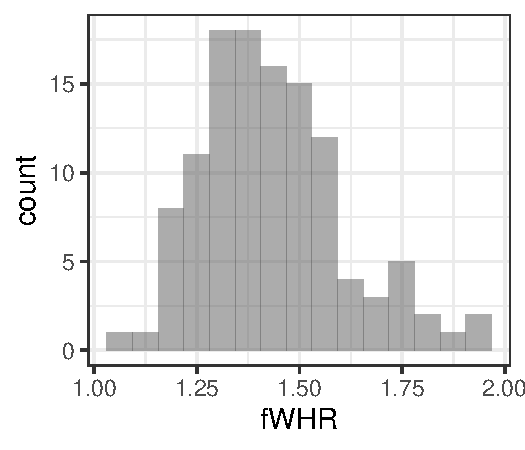
\includegraphics{bookdown-demo_files/figure-latex/view-data-1.pdf} 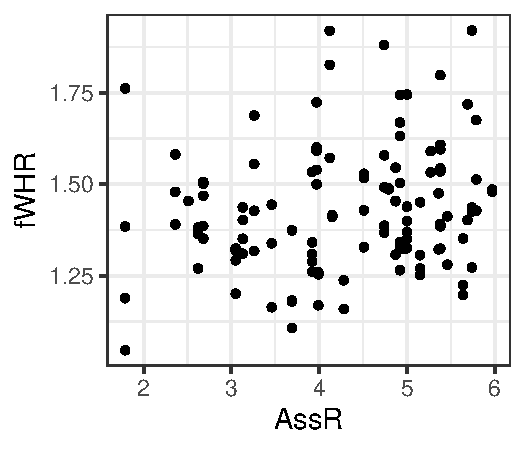
\includegraphics{bookdown-demo_files/figure-latex/view-data-2.pdf}

\hypertarget{simple-linear-regression-residuals-least-squares}{%
\section{Simple linear regression, Residuals \& Least squares}\label{simple-linear-regression-residuals-least-squares}}

First, let's review and consider a simple (one-predictor) linear regression model. Fit the model

\begin{Shaded}
\begin{Highlighting}[]
\NormalTok{slr <-}\StringTok{ }\KeywordTok{lm}\NormalTok{(fWHR }\OperatorTok{~}\StringTok{ }\NormalTok{AssR, }\DataTypeTok{data=}\NormalTok{bonobos)}
\end{Highlighting}
\end{Shaded}

Extract the slope and intercept values:

\begin{Shaded}
\begin{Highlighting}[]
\KeywordTok{coef}\NormalTok{(slr)}
\end{Highlighting}
\end{Shaded}

\begin{verbatim}
## (Intercept)        AssR 
##  1.30685287  0.02918242
\end{verbatim}

Add the regression line to the plot:

\begin{Shaded}
\begin{Highlighting}[]
\KeywordTok{gf_point}\NormalTok{(fWHR }\OperatorTok{~}\StringTok{ }\NormalTok{AssR, }\DataTypeTok{data=}\NormalTok{bonobos) }\OperatorTok\StringTok{ }
\StringTok{  }\KeywordTok{gf_lm}\NormalTok{()}
\end{Highlighting}
\end{Shaded}

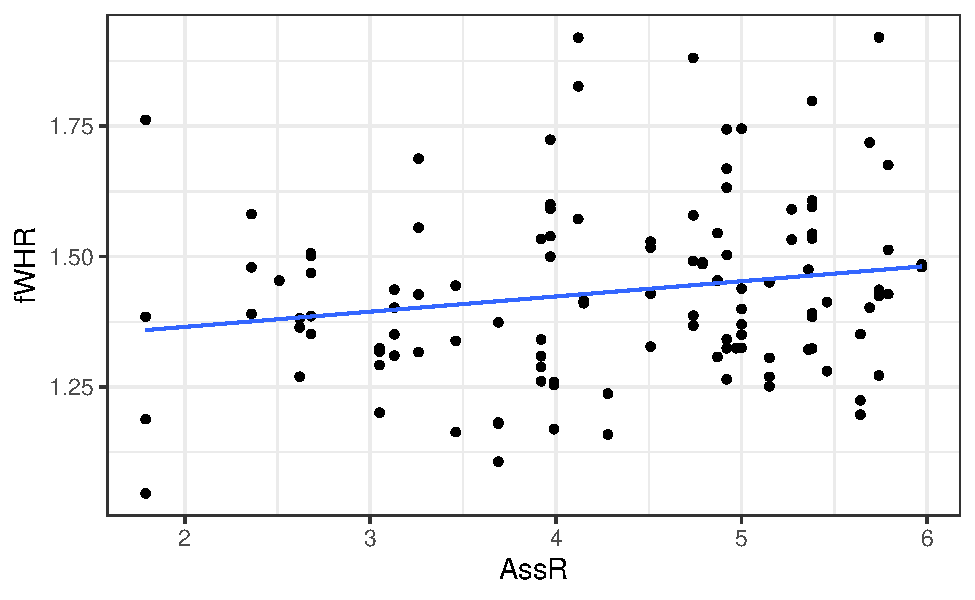
\includegraphics{bookdown-demo_files/figure-latex/lm-scatter-with-line-1.pdf}

\begin{Shaded}
\begin{Highlighting}[]
\KeywordTok{summary}\NormalTok{(slr)}
\end{Highlighting}
\end{Shaded}

\begin{verbatim}
## 
## Call:
## lm(formula = fWHR ~ AssR, data = bonobos)
## 
## Residuals:
##      Min       1Q   Median       3Q      Max 
## -0.31320 -0.11369 -0.01242  0.09008  0.49241 
## 
## Coefficients:
##             Estimate Std. Error t value Pr(>|t|)    
## (Intercept)  1.30685    0.06283  20.801   <2e-16 ***
## AssR         0.02918    0.01420   2.055   0.0421 *  
## ---
## Signif. codes:  0 '***' 0.001 '**' 0.01 '*' 0.05 '.' 0.1 ' ' 1
## 
## Residual standard error: 0.1689 on 115 degrees of freedom
## Multiple R-squared:  0.03542,    Adjusted R-squared:  0.02704 
## F-statistic: 4.223 on 1 and 115 DF,  p-value: 0.04213
\end{verbatim}

\hypertarget{using-lm-to-fit-a-linear-regression-in-r}{%
\subsection{\texorpdfstring{Using \texttt{lm()} to fit a linear regression in R}{Using lm() to fit a linear regression in R}}\label{using-lm-to-fit-a-linear-regression-in-r}}

\hypertarget{equation-of-the-fitted-regression-line}{%
\subsection{Equation of the fitted regression line}\label{equation-of-the-fitted-regression-line}}

\hypertarget{multiple-regression}{%
\section{Multiple regression}\label{multiple-regression}}

Rarely does our response variable \textbf{really} depend on only one predictor. Can we improve the model by adding more predictors?

\begin{Shaded}
\begin{Highlighting}[]
\NormalTok{mlr <-}\StringTok{ }\KeywordTok{lm}\NormalTok{(fWHR }\OperatorTok{~}\StringTok{ }\NormalTok{AssR }\OperatorTok{+}\StringTok{ }\NormalTok{weight, }\DataTypeTok{data=}\NormalTok{bonobos)}
\KeywordTok{coef}\NormalTok{(mlr)}
\end{Highlighting}
\end{Shaded}

\begin{verbatim}
## (Intercept)        AssR      weight 
## 0.944790930 0.039888045 0.008644299
\end{verbatim}

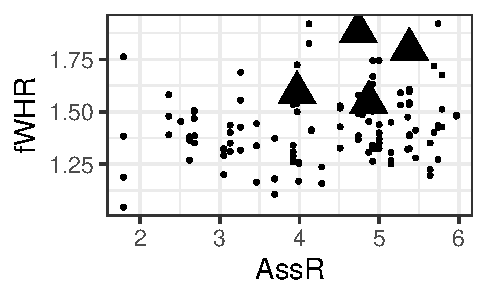
\includegraphics{bookdown-demo_files/figure-latex/mult-reg-plots-1.pdf} 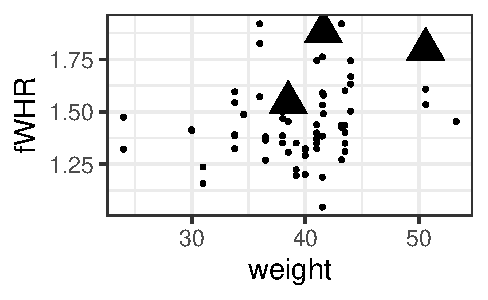
\includegraphics{bookdown-demo_files/figure-latex/mult-reg-plots-2.pdf}

\hypertarget{is-it-really-better}{%
\subsection{Is it really better?}\label{is-it-really-better}}

How do we know if the model with more predictors is ``better''? (For a more detailed answer, wait about a week\ldots) But before we can define a ``beter'' model: how did R find the ``best'' intercept and slopes?

\hypertarget{regression-residuals-errors}{%
\subsection{Regression residuals = ``errors''}\label{regression-residuals-errors}}

\hypertarget{computing-predictions}{%
\subsection{Computing Predictions}\label{computing-predictions}}

Use the regression equation to compute \textbf{predicted values} for the three data points below:

\begin{verbatim}
##        fWHR AssR weight
## 8  1.880866 4.74   41.6
## 25 1.798387 5.38   50.6
## 41 1.591440 3.97     NA
## 65 1.545019 4.87   38.5
\end{verbatim}

\hypertarget{predictors-with-two-categories}{%
\section{Predictors with two categories}\label{predictors-with-two-categories}}

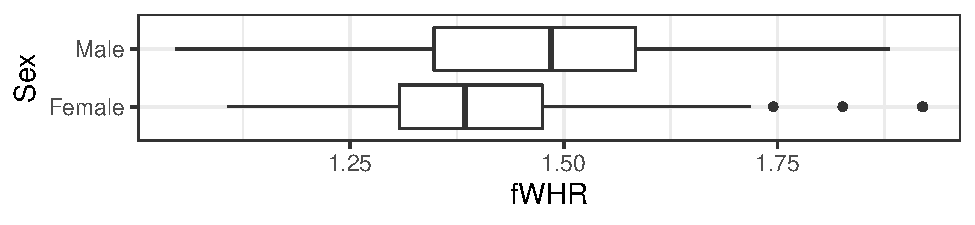
\includegraphics{bookdown-demo_files/figure-latex/unnamed-chunk-2-1.pdf}

\begin{Shaded}
\begin{Highlighting}[]
\NormalTok{mlr2 <-}\StringTok{ }\KeywordTok{lm}\NormalTok{(fWHR }\OperatorTok{~}\StringTok{ }\NormalTok{AssR }\OperatorTok{+}\StringTok{ }\NormalTok{weight }\OperatorTok{+}\StringTok{ }\NormalTok{Sex, }\DataTypeTok{data =}\NormalTok{ bonobos)}
\KeywordTok{coef}\NormalTok{(mlr2)}
\end{Highlighting}
\end{Shaded}

\begin{verbatim}
## (Intercept)        AssR      weight     SexMale 
## 1.065420976 0.058435841 0.002257142 0.128484275
\end{verbatim}

How does the model incorporate this covariate mathematically?

\hypertarget{predictors-with-more-categories}{%
\subsection{Predictors with more categories}\label{predictors-with-more-categories}}

\begin{Shaded}
\begin{Highlighting}[]
\KeywordTok{gf_boxplot}\NormalTok{(fWHR }\OperatorTok{~}\StringTok{ }\NormalTok{Group, }\DataTypeTok{data =}\NormalTok{ bonobos)}
\end{Highlighting}
\end{Shaded}

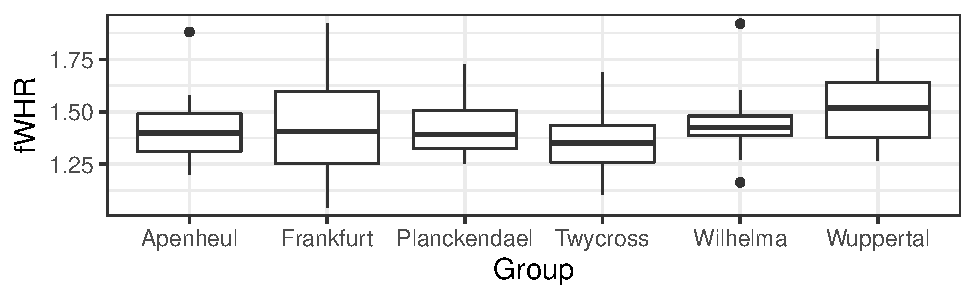
\includegraphics{bookdown-demo_files/figure-latex/unnamed-chunk-4-1.pdf}

\begin{Shaded}
\begin{Highlighting}[]
\NormalTok{mlr3 <-}\StringTok{ }\KeywordTok{lm}\NormalTok{(fWHR }\OperatorTok{~}\StringTok{ }\NormalTok{AssR }\OperatorTok{+}\StringTok{ }\NormalTok{weight }\OperatorTok{+}\StringTok{ }\NormalTok{Sex }\OperatorTok{+}\StringTok{ }\NormalTok{Group, }\DataTypeTok{data =}\NormalTok{ bonobos)}
\KeywordTok{coef}\NormalTok{(mlr3)}
\end{Highlighting}
\end{Shaded}

\begin{verbatim}
##       (Intercept)              AssR            weight           SexMale 
##       1.007734691       0.064361973       0.003458979       0.124854271 
##    GroupFrankfurt GroupPlanckendael     GroupTwycross     GroupWilhelma 
##       0.037426358      -0.008464572      -0.112907589       0.011186724 
##    GroupWuppertal 
##      -0.004364826
\end{verbatim}

How does the model incorporate \textbf{this} covariate mathematically?

\hypertarget{returning-to-the-r-model-summary}{%
\section{Returning to the R Model Summary}\label{returning-to-the-r-model-summary}}

There are several bits of information you should be able to extract from the \texttt{summary()} output R produces on a fitted linear regression model:

\begin{itemize}
\item
  \(\beta\)s, Coefficient Estimates
\item
  \(\sigma\), labeled ``residual standard error''
\item
  \(R^2\) (adjusted)
\end{itemize}

\begin{Shaded}
\begin{Highlighting}[]
\NormalTok{mlr3 <-}\StringTok{ }\KeywordTok{lm}\NormalTok{(fWHR }\OperatorTok{~}\StringTok{ }\NormalTok{AssR }\OperatorTok{+}\StringTok{ }\NormalTok{weight }\OperatorTok{+}\StringTok{ }\NormalTok{Sex }\OperatorTok{+}\StringTok{ }\NormalTok{Group, }\DataTypeTok{data =}\NormalTok{ bonobos)}
\KeywordTok{summary}\NormalTok{(mlr3)}
\end{Highlighting}
\end{Shaded}

\begin{verbatim}
## 
## Call:
## lm(formula = fWHR ~ AssR + weight + Sex + Group, data = bonobos)
## 
## Residuals:
##      Min       1Q   Median       3Q      Max 
## -0.38288 -0.09488 -0.02642  0.07196  0.48464 
## 
## Coefficients:
##                    Estimate Std. Error t value Pr(>|t|)    
## (Intercept)        1.007735   0.217585   4.631 2.05e-05 ***
## AssR               0.064362   0.021158   3.042   0.0035 ** 
## weight             0.003459   0.005547   0.624   0.5353    
## SexMale            0.124854   0.059278   2.106   0.0394 *  
## GroupFrankfurt     0.037426   0.074892   0.500   0.6191    
## GroupPlanckendael -0.008465   0.075407  -0.112   0.9110    
## GroupTwycross     -0.112908   0.074779  -1.510   0.1364    
## GroupWilhelma      0.011187   0.085538   0.131   0.8964    
## GroupWuppertal    -0.004365   0.071292  -0.061   0.9514    
## ---
## Signif. codes:  0 '***' 0.001 '**' 0.01 '*' 0.05 '.' 0.1 ' ' 1
## 
## Residual standard error: 0.1691 on 59 degrees of freedom
##   (49 observations deleted due to missingness)
## Multiple R-squared:  0.2517, Adjusted R-squared:  0.1502 
## F-statistic:  2.48 on 8 and 59 DF,  p-value: 0.02167
\end{verbatim}

\hypertarget{predictions-from-the-model}{%
\section{Predictions from the model}\label{predictions-from-the-model}}

\hypertarget{by-hand}{%
\subsection{By Hand}\label{by-hand}}

The equation for the fitted model above is:

\[ y = \beta_0 + \beta_1x_1 + \beta_2x_2 + \beta_3I_{Male} + \beta_4I_{Frankfurt} + \beta_5I_{Planckendael} + \beta_6I_{Twycross} + \beta_7I_{Wilhelma} + \beta_7I_{Wuppertal} + \epsilon\]

where

\begin{itemize}
\tightlist
\item
  \(y =\)
\item
  \(\beta_0=\)
\end{itemize}

\begin{itemize}
\tightlist
\item
  \(x_1=\)
\item
  \(x_2=\)
\item
  \(\beta_1, \beta_2, \beta_3 ...\) are:
\item
  \(I_{Male} =\)
\item
  \(I_{Frankfurt} =\)
\item
  \(I_{Planckendael} =\) \hspace{3in}, etc.
\item
  \(\epsilon=\)
\end{itemize}

\hypertarget{comprehension-check}{%
\subsubsection{Comprehension check:}\label{comprehension-check}}

What is the expected fWHR (according to this model) for a 30 kg female bonobo at the Wilhelma zoo?

\hypertarget{prediction-plots-in-r}{%
\subsection{Prediction Plots in R}\label{prediction-plots-in-r}}

We can ask R to compute predictions for \textbf{all} the data points in the real dataset.

\begin{Shaded}
\begin{Highlighting}[]
\NormalTok{bonobos <-}\StringTok{ }\NormalTok{bonobos }\OperatorTok\StringTok{ }
\StringTok{  }\KeywordTok{mutate}\NormalTok{(}\DataTypeTok{preds =} \KeywordTok{predict}\NormalTok{(mlr3))}
\end{Highlighting}
\end{Shaded}

\begin{verbatim}
## Error: Column `preds` must be length 117 (the number of rows) or one, not 68
\end{verbatim}

Wait, what? This error is because the \texttt{lm()} function removes rows containing missing values from the dataset, so it computes only 68 residuals (for the complete cases in the data). This doesn't match the 117 rows in the original data. We can solve the problem by omitting rows with missing values first. To be safe, we first select only the variables we need, so we don't omit rows based on missing values in unused variables.

\begin{Shaded}
\begin{Highlighting}[]
\NormalTok{b2 <-}\StringTok{ }\NormalTok{bonobos }\OperatorTok
\StringTok{  }\NormalTok{dplyr}\OperatorTok{::}\KeywordTok{select}\NormalTok{(fWHR, weight, AssR, Sex, Group) }\OperatorTok
\StringTok{  }\KeywordTok{na.omit}\NormalTok{() }\OperatorTok
\StringTok{  }\KeywordTok{mutate}\NormalTok{(}\DataTypeTok{preds =} \KeywordTok{predict}\NormalTok{(mlr3))}
\end{Highlighting}
\end{Shaded}

\emph{We have a full set of predictions!}

But if we plot these predictions on a scatter plot of \texttt{fWHR} as a function of \texttt{AssR}, we \emph{do not} get a straight line, because the predictions are also impacted by varying values of \texttt{weight}, \texttt{Sex}, and \texttt{Group}:

\begin{Shaded}
\begin{Highlighting}[]
\KeywordTok{gf_point}\NormalTok{(fWHR }\OperatorTok{~}\StringTok{ }\NormalTok{AssR, }\DataTypeTok{data =}\NormalTok{ b2) }\OperatorTok
\StringTok{  }\KeywordTok{gf_line}\NormalTok{(preds }\OperatorTok{~}\StringTok{ }\NormalTok{AssR, }\DataTypeTok{data=}\NormalTok{b2)}
\end{Highlighting}
\end{Shaded}

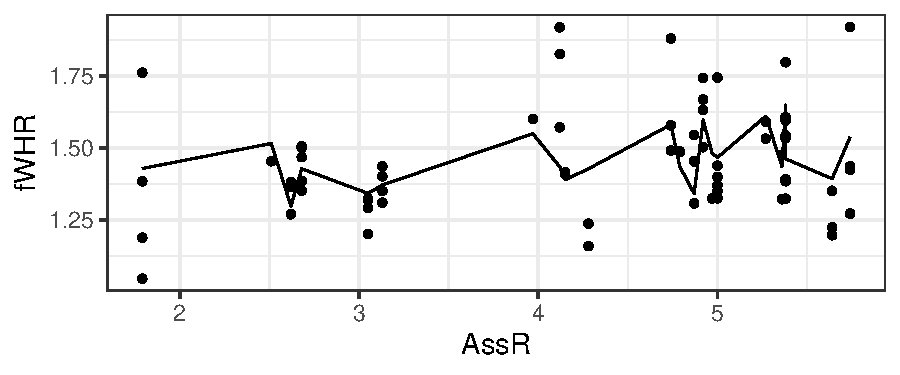
\includegraphics{bookdown-demo_files/figure-latex/unnamed-chunk-8-1.pdf}

\emph{But\ldots we would really like a straight line that helps us visualize the meaning of the \(\beta\) (slope coefficient) for \texttt{AssR}.} We can make predictions for a \textbf{hypothetical} dataset, in which \texttt{AssR} varies over a reasonable range, but the other predictors stay constant. This lets us see how \texttt{AssR} (and only \texttt{AssR}) affects the response, without contributions from other predictors. In choosing the values to include in hypothetical dataset, we often choose to hold variables constant at their most common or median values, but not blindly: also, avoid impossible or implausible variable combinations (for example, specifying that a person lives in the state of Michigan but the city of Chicago, or that they are a 5-year-old person with 4 children). \emph{In this case, to match the figures in the published paper, we are also going to vary the \texttt{Sex} - but generally you'd only allow one predictor to vary.}

\begin{Shaded}
\begin{Highlighting}[]
\NormalTok{fake_data <-}\StringTok{ }\KeywordTok{expand.grid}\NormalTok{(}\DataTypeTok{AssR =} \KeywordTok{seq}\NormalTok{(}\DataTypeTok{from=}\FloatTok{1.8}\NormalTok{, }\DataTypeTok{to=}\FloatTok{5.7}\NormalTok{, }\DataTypeTok{by=}\FloatTok{0.05}\NormalTok{),}
                         \DataTypeTok{weight =} \FloatTok{38.5}\NormalTok{,}
                         \DataTypeTok{Sex =} \KeywordTok{c}\NormalTok{(}\StringTok{'Female'}\NormalTok{, }\StringTok{'Male'}\NormalTok{),}
                         \DataTypeTok{Group =} \StringTok{'Wuppertal'}\NormalTok{)}

\NormalTok{fake_data <-}\StringTok{ }\NormalTok{fake_data }\OperatorTok\StringTok{ }
\StringTok{  }\KeywordTok{mutate}\NormalTok{(}\DataTypeTok{preds =} \KeywordTok{predict}\NormalTok{(mlr3, }\DataTypeTok{newdata =}\NormalTok{ fake_data))}
\KeywordTok{gf_line}\NormalTok{(preds }\OperatorTok{~}\StringTok{ }\NormalTok{AssR, }\DataTypeTok{color =} \OperatorTok{~}\NormalTok{Sex, }\DataTypeTok{data=}\NormalTok{fake_data) }\OperatorTok\StringTok{ }\KeywordTok{gf_labs}\NormalTok{(}\DataTypeTok{y=}\StringTok{'Predicted}\CharTok{\textbackslash{}n}\StringTok{fWHR'}\NormalTok{)}
\end{Highlighting}
\end{Shaded}

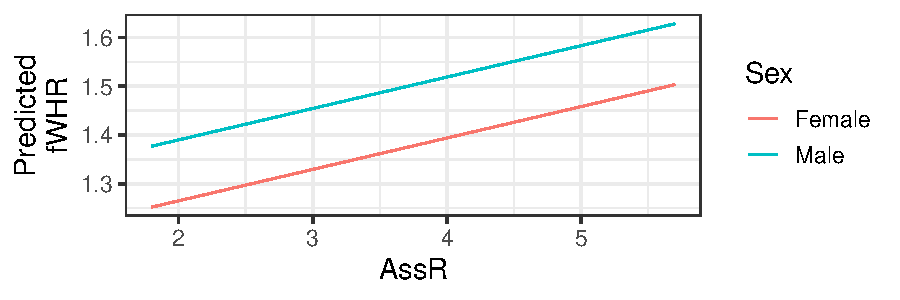
\includegraphics{bookdown-demo_files/figure-latex/unnamed-chunk-9-1.pdf}

\hypertarget{comprehension-checks}{%
\subsubsection{Comprehension checks:}\label{comprehension-checks}}

\begin{itemize}
\tightlist
\item
  Should we overlay prediction-plot line(s) on the data scatter plot?
\item
  How do you think the plot would look if we changed the constant predictor values?
\item
  What is missing from this picture?
\end{itemize}

\hypertarget{shortcut}{%
\subsubsection{Shortcut}\label{shortcut}}

\begin{Shaded}
\begin{Highlighting}[]
\KeywordTok{require}\NormalTok{(s245)}
\KeywordTok{pred_plot}\NormalTok{(mlr3, }\StringTok{'AssR'}\NormalTok{)}
\end{Highlighting}
\end{Shaded}

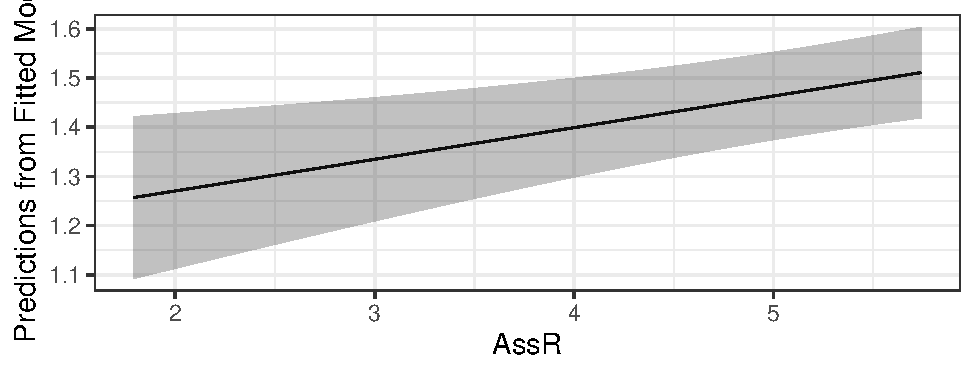
\includegraphics{bookdown-demo_files/figure-latex/unnamed-chunk-10-1.pdf}

\hypertarget{why-are-we-doing-this-again}{%
\section{Why are we doing this again?}\label{why-are-we-doing-this-again}}

Why make prediction plots?

\hypertarget{shortcut-method---with-uncertainty}{%
\section{Shortcut Method - With Uncertainty}\label{shortcut-method---with-uncertainty}}

We saw before that \texttt{pred\_plot()} makes it very easy for us to generate prediction plots showing what a (multiple regression) model says about the relationship between the response and \emph{one} of the predictors:

\begin{Shaded}
\begin{Highlighting}[]
\KeywordTok{require}\NormalTok{(s245)}
\KeywordTok{pred_plot}\NormalTok{(mlr3, }\StringTok{'AssR'}\NormalTok{) }\OperatorTok
\StringTok{  }\KeywordTok{gf_labs}\NormalTok{(}\DataTypeTok{y =} \StringTok{'Predicted fWHR'}\NormalTok{)}
\end{Highlighting}
\end{Shaded}

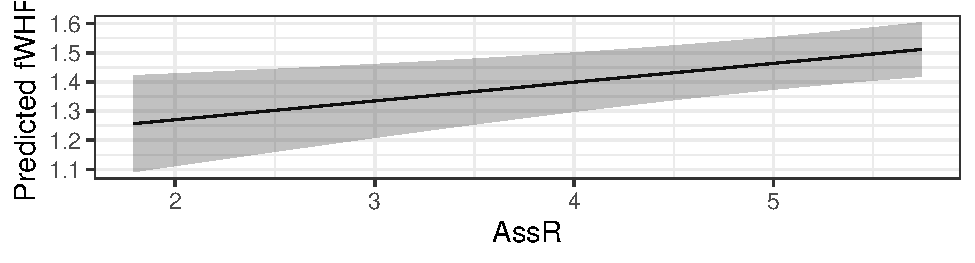
\includegraphics{bookdown-demo_files/figure-latex/unnamed-chunk-11-1.pdf}

\emph{Note the custom axis label - otherwise you get a long, unwieldy default ``Predictions from fitted model''}

\begin{Shaded}
\begin{Highlighting}[]
\KeywordTok{require}\NormalTok{(s245)}
\KeywordTok{pred_plot}\NormalTok{(mlr3, }\StringTok{'Group'}\NormalTok{) }\OperatorTok
\StringTok{  }\KeywordTok{gf_labs}\NormalTok{(}\DataTypeTok{y =} \StringTok{'Predicted fWHR'}\NormalTok{)}
\end{Highlighting}
\end{Shaded}

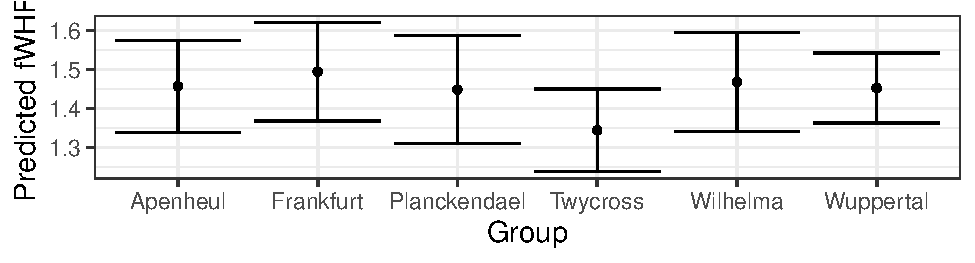
\includegraphics{bookdown-demo_files/figure-latex/unnamed-chunk-12-1.pdf}

They look nice! But they should raise two questions:

\begin{itemize}
\item
  Uncertainty:
\item
  Fixed values:
\end{itemize}

\begin{Shaded}
\begin{Highlighting}[]
\KeywordTok{get_fixed}\NormalTok{(bonobos)  }\OperatorTok\StringTok{ }
\StringTok{  }\NormalTok{pander}\OperatorTok{::}\KeywordTok{pander}\NormalTok{()}
\end{Highlighting}
\end{Shaded}

\begin{longtable}[]{@{}cccccccccc@{}}
\toprule
\begin{minipage}[b]{0.06\columnwidth}\centering
Name\strut
\end{minipage} & \begin{minipage}[b]{0.10\columnwidth}\centering
Group\strut
\end{minipage} & \begin{minipage}[b]{0.08\columnwidth}\centering
Sex\strut
\end{minipage} & \begin{minipage}[b]{0.05\columnwidth}\centering
Age\strut
\end{minipage} & \begin{minipage}[b]{0.07\columnwidth}\centering
fWHR\strut
\end{minipage} & \begin{minipage}[b]{0.06\columnwidth}\centering
AssR\strut
\end{minipage} & \begin{minipage}[b]{0.08\columnwidth}\centering
normDS\strut
\end{minipage} & \begin{minipage}[b]{0.08\columnwidth}\centering
weight\strut
\end{minipage} & \begin{minipage}[b]{0.07\columnwidth}\centering
three\strut
\end{minipage} & \begin{minipage}[b]{0.09\columnwidth}\centering
pt\_size\strut
\end{minipage}\tabularnewline
\midrule
\endhead
\begin{minipage}[t]{0.06\columnwidth}\centering
Eja\strut
\end{minipage} & \begin{minipage}[t]{0.10\columnwidth}\centering
Twycross\strut
\end{minipage} & \begin{minipage}[t]{0.08\columnwidth}\centering
Female\strut
\end{minipage} & \begin{minipage}[t]{0.05\columnwidth}\centering
21\strut
\end{minipage} & \begin{minipage}[t]{0.07\columnwidth}\centering
1.412\strut
\end{minipage} & \begin{minipage}[t]{0.06\columnwidth}\centering
4.51\strut
\end{minipage} & \begin{minipage}[t]{0.08\columnwidth}\centering
2.368\strut
\end{minipage} & \begin{minipage}[t]{0.08\columnwidth}\centering
40\strut
\end{minipage} & \begin{minipage}[t]{0.07\columnwidth}\centering
no\strut
\end{minipage} & \begin{minipage}[t]{0.09\columnwidth}\centering
1\strut
\end{minipage}\tabularnewline
\bottomrule
\end{longtable}

\hypertarget{anatomy-of-a-confidence-interval}{%
\subsection{Anatomy of a Confidence Interval}\label{anatomy-of-a-confidence-interval}}

\begin{Shaded}
\begin{Highlighting}[]
\KeywordTok{pred_plot}\NormalTok{(mlr3, }\StringTok{'Sex'}\NormalTok{) }\OperatorTok
\StringTok{  }\KeywordTok{gf_labs}\NormalTok{(}\DataTypeTok{y =} \StringTok{'Predicted fWHR'}\NormalTok{)}
\end{Highlighting}
\end{Shaded}

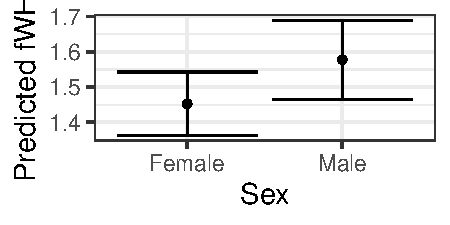
\includegraphics{bookdown-demo_files/figure-latex/unnamed-chunk-14-1.pdf}

\hypertarget{diy-method}{%
\section{DIY Method}\label{diy-method}}

\hypertarget{creating-a-hypothetical-dataset}{%
\subsection{Creating a hypothetical dataset}\label{creating-a-hypothetical-dataset}}

We would like to create a hypothetical dataset where one predictor variable varies, and all the rest stay fixed. Let's choose \texttt{AssR}. We use \texttt{expand.grid()}:

\begin{Shaded}
\begin{Highlighting}[]
\NormalTok{fake_data <-}\StringTok{ }\KeywordTok{expand.grid}\NormalTok{(}\DataTypeTok{AssR =} \KeywordTok{seq}\NormalTok{(}\DataTypeTok{from=}\FloatTok{1.8}\NormalTok{, }\DataTypeTok{to=}\FloatTok{5.7}\NormalTok{, }\DataTypeTok{by=}\FloatTok{0.05}\NormalTok{),}
                         \DataTypeTok{weight =} \DecValTok{40}\NormalTok{,}
                         \DataTypeTok{Sex =} \StringTok{'Female'}\NormalTok{,}
                         \DataTypeTok{Group =} \StringTok{'Twycross'}\NormalTok{)}
\KeywordTok{glimpse}\NormalTok{(fake_data)}
\end{Highlighting}
\end{Shaded}

\begin{verbatim}
## Observations: 79
## Variables: 4
## $ AssR   <dbl> 1.80, 1.85, 1.90, 1.95, 2.00, 2.05, 2.10, 2.15, 2.20, 2...
## $ weight <dbl> 40, 40, 40, 40, 40, 40, 40, 40, 40, 40, 40, 40, 40, 40,...
## $ Sex    <fct> Female, Female, Female, Female, Female, Female, Female,...
## $ Group  <fct> Twycross, Twycross, Twycross, Twycross, Twycross, Twycr...
\end{verbatim}

Now, make predictions for our fake data.

\begin{Shaded}
\begin{Highlighting}[]
\NormalTok{preds <-}\StringTok{ }\KeywordTok{predict}\NormalTok{(mlr3, }\DataTypeTok{newdata =}\NormalTok{ fake_data, }\DataTypeTok{se.fit =} \OtherTok{TRUE}\NormalTok{)}
\NormalTok{fake_data <-}\StringTok{ }\NormalTok{fake_data }\OperatorTok
\StringTok{  }\KeywordTok{mutate}\NormalTok{(}\DataTypeTok{fitted =}\NormalTok{ preds}\OperatorTok{$}\NormalTok{fit,}
         \DataTypeTok{se.fit =}\NormalTok{ preds}\OperatorTok{$}\NormalTok{se.fit)}
\KeywordTok{glimpse}\NormalTok{(fake_data)}
\end{Highlighting}
\end{Shaded}

\begin{verbatim}
## Observations: 79
## Variables: 6
## $ AssR   <dbl> 1.80, 1.85, 1.90, 1.95, 2.00, 2.05, 2.10, 2.15, 2.20, 2...
## $ weight <dbl> 40, 40, 40, 40, 40, 40, 40, 40, 40, 40, 40, 40, 40, 40,...
## $ Sex    <fct> Female, Female, Female, Female, Female, Female, Female,...
## $ Group  <fct> Twycross, Twycross, Twycross, Twycross, Twycross, Twycr...
## $ fitted <dbl> 1.149038, 1.152256, 1.155474, 1.158692, 1.161910, 1.165...
## $ se.fit <dbl> 0.08347207, 0.08267088, 0.08187552, 0.08108616, 0.08030...
\end{verbatim}

How do we go from \emph{standard errors} to \emph{confidence intervals}? We can either do this before plotting, or while plotting. To do it before and add the results to the hypothetical dataset:

\begin{Shaded}
\begin{Highlighting}[]
\NormalTok{fake_data <-}\StringTok{ }\NormalTok{fake_data }\OperatorTok
\StringTok{  }\KeywordTok{mutate}\NormalTok{(}\DataTypeTok{CI_lower =}\NormalTok{ fitted }\OperatorTok{-}\StringTok{ }\FloatTok{1.96}\OperatorTok{*}\NormalTok{se.fit,}
         \DataTypeTok{CI_upper =}\NormalTok{ fitted }\OperatorTok{+}\StringTok{ }\FloatTok{1.96}\OperatorTok{*}\NormalTok{se.fit)}
\KeywordTok{glimpse}\NormalTok{(fake_data)}
\end{Highlighting}
\end{Shaded}

\begin{verbatim}
## Observations: 79
## Variables: 8
## $ AssR     <dbl> 1.80, 1.85, 1.90, 1.95, 2.00, 2.05, 2.10, 2.15, 2.20,...
## $ weight   <dbl> 40, 40, 40, 40, 40, 40, 40, 40, 40, 40, 40, 40, 40, 4...
## $ Sex      <fct> Female, Female, Female, Female, Female, Female, Femal...
## $ Group    <fct> Twycross, Twycross, Twycross, Twycross, Twycross, Twy...
## $ fitted   <dbl> 1.149038, 1.152256, 1.155474, 1.158692, 1.161910, 1.1...
## $ se.fit   <dbl> 0.08347207, 0.08267088, 0.08187552, 0.08108616, 0.080...
## $ CI_lower <dbl> 0.9854326, 0.9902210, 0.9949980, 0.9997632, 1.0045164...
## $ CI_upper <dbl> 1.312643, 1.314291, 1.315950, 1.317621, 1.319304, 1.3...
\end{verbatim}

\hypertarget{making-the-plot}{%
\subsection{Making the plot}\label{making-the-plot}}

Now, we just need to plot!

\begin{Shaded}
\begin{Highlighting}[]
\KeywordTok{gf_line}\NormalTok{(fitted }\OperatorTok{~}\StringTok{ }\NormalTok{AssR, }\DataTypeTok{data=}\NormalTok{fake_data) }\OperatorTok\StringTok{ }
\StringTok{  }\KeywordTok{gf_labs}\NormalTok{(}\DataTypeTok{y=}\StringTok{'Predicted}\CharTok{\textbackslash{}n}\StringTok{fWHR'}\NormalTok{) }\OperatorTok
\StringTok{  }\KeywordTok{gf_ribbon}\NormalTok{(CI_lower }\OperatorTok{+}\StringTok{ }\NormalTok{CI_upper }\OperatorTok{~}\StringTok{ }\NormalTok{AssR, }\DataTypeTok{data =}\NormalTok{ fake_data)}
\end{Highlighting}
\end{Shaded}

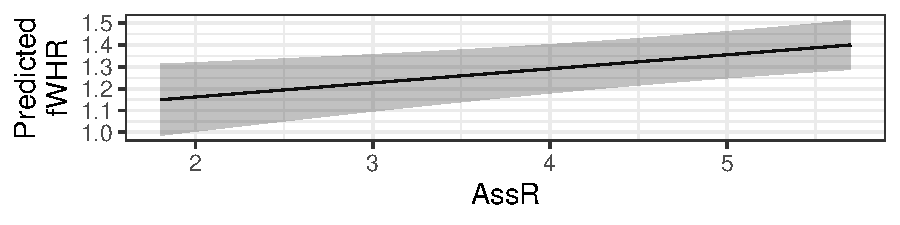
\includegraphics{bookdown-demo_files/figure-latex/unnamed-chunk-18-1.pdf}

If we wanted to figure out the CI bounds \emph{while} plotting, we could calculate them on the fly like this:

\begin{Shaded}
\begin{Highlighting}[]
\KeywordTok{gf_line}\NormalTok{(fitted }\OperatorTok{~}\StringTok{ }\NormalTok{AssR, }\DataTypeTok{data=}\NormalTok{fake_data) }\OperatorTok\StringTok{ }
\StringTok{  }\KeywordTok{gf_labs}\NormalTok{(}\DataTypeTok{y=}\StringTok{'Predicted}\CharTok{\textbackslash{}n}\StringTok{fWHR'}\NormalTok{) }\OperatorTok
\StringTok{  }\KeywordTok{gf_ribbon}\NormalTok{((fitted }\OperatorTok{-}\StringTok{ }\FloatTok{1.96}\OperatorTok{*}\NormalTok{se.fit ) }\OperatorTok{+}\StringTok{ }\NormalTok{(fitted }\OperatorTok{+}\StringTok{ }\FloatTok{1.96}\OperatorTok{*}\NormalTok{se.fit) }\OperatorTok{~}\StringTok{ }\NormalTok{AssR,}
            \DataTypeTok{data =}\NormalTok{ fake_data)}
\end{Highlighting}
\end{Shaded}

(which will look just the same).

\hypertarget{categorical-predictors}{%
\subsection{Categorical predictors}\label{categorical-predictors}}

What will be different if the predictor of interest is \emph{categorical}?

\begin{itemize}
\item
  hypothetical data:
\item
  plot:
\end{itemize}

\begin{Shaded}
\begin{Highlighting}[]
\NormalTok{fake_sex_data <-}\StringTok{ }\KeywordTok{expand.grid}\NormalTok{(}\DataTypeTok{AssR =} \FloatTok{4.51}\NormalTok{,}
                         \DataTypeTok{weight =} \DecValTok{40}\NormalTok{,}
                         \DataTypeTok{Sex =} \KeywordTok{c}\NormalTok{(}\StringTok{'Male'}\NormalTok{, }\StringTok{'Female'}\NormalTok{),}
                         \DataTypeTok{Group =} \StringTok{'Twycross'}\NormalTok{)}
\NormalTok{preds <-}\StringTok{ }\KeywordTok{predict}\NormalTok{(mlr3, }\DataTypeTok{newdata =}\NormalTok{ fake_sex_data, }\DataTypeTok{se.fit =} \OtherTok{TRUE}\NormalTok{)}
\NormalTok{fake_sex_data <-}\StringTok{ }\NormalTok{fake_sex_data }\OperatorTok
\StringTok{  }\KeywordTok{mutate}\NormalTok{(}\DataTypeTok{fitted =}\NormalTok{ preds}\OperatorTok{$}\NormalTok{fit,}
         \DataTypeTok{se.fit =}\NormalTok{ preds}\OperatorTok{$}\NormalTok{se.fit)}
\KeywordTok{gf_point}\NormalTok{(fitted }\OperatorTok{~}\StringTok{ }\NormalTok{Sex, }\DataTypeTok{data=}\NormalTok{fake_sex_data) }\OperatorTok\StringTok{ }
\StringTok{  }\KeywordTok{gf_labs}\NormalTok{(}\DataTypeTok{y=}\StringTok{'Predicted fWHR'}\NormalTok{) }\OperatorTok
\StringTok{  }\KeywordTok{gf_errorbar}\NormalTok{((fitted }\OperatorTok{-}\StringTok{ }\FloatTok{1.96}\OperatorTok{*}\NormalTok{se.fit ) }\OperatorTok{+}\StringTok{ }\NormalTok{(fitted }\OperatorTok{+}\StringTok{ }\FloatTok{1.96}\OperatorTok{*}\NormalTok{se.fit) }\OperatorTok{~}\StringTok{ }\NormalTok{Sex, }
            \DataTypeTok{data =}\NormalTok{ fake_sex_data)}
\end{Highlighting}
\end{Shaded}

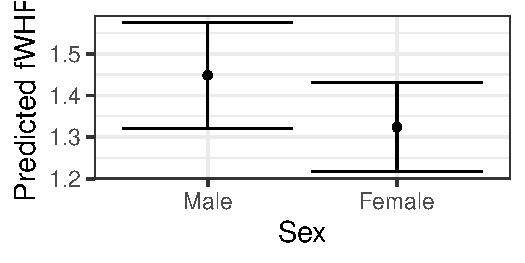
\includegraphics{bookdown-demo_files/figure-latex/unnamed-chunk-20-1.pdf}

\hypertarget{model-selection-using-information-criteria}{%
\chapter{Model Selection Using Information Criteria}\label{model-selection-using-information-criteria}}

So far, we have learned to fit models with multiple predictors, both quantitative and categorical, and to assess whether required conditions are met for linear regression to be an appropriate model for a dataset.

One missing piece is: If I have an appropriate model with a set of multiple predictors, how can I choose which predictors are worth retaining in a ``best'' model for the data (and which ones have no relationship, or a weak relationship, with the response, so should be discarded)?

\hypertarget{data-and-model}{%
\section{Data and Model}\label{data-and-model}}

Today we will recreate part of the analysis from \href{https://doi.org/10.1111/1365-2664.12798}{\emph{Vertebrate community composition and diversity declines along a defaunation gradient radiating from rural villages in Gabon}}, by Sally Koerner and colleagues. They investigated the relationship between rural villages, hunting, and wildlife in Gabon. They asked how monkey abundance depends on distance from villages, village size, and vegetation characteristics. They shared their data at \href{https://datadryad.org/stash/dataset/doi:10.5061/dryad.vs97g}{Dryad.org} and we can read it in and fit a regression model like this:

\begin{Shaded}
\begin{Highlighting}[]
\NormalTok{defaun <-}\StringTok{ }\KeywordTok{read.csv}\NormalTok{(}\StringTok{'http://sldr.netlify.com/data/koerner_gabon_defaunation.csv'}\NormalTok{)}
\end{Highlighting}
\end{Shaded}

\begin{Shaded}
\begin{Highlighting}[]
\NormalTok{ape_mod <-}\StringTok{ }\KeywordTok{lm}\NormalTok{(RA_Apes }\OperatorTok{~}\StringTok{ }\NormalTok{Veg_DBH }\OperatorTok{+}\StringTok{ }\NormalTok{Veg_Canopy }\OperatorTok{+}\StringTok{ }\NormalTok{Veg_Understory }\OperatorTok{+}
\StringTok{                   }\NormalTok{Veg_Rich }\OperatorTok{+}\StringTok{ }\NormalTok{Veg_Stems }\OperatorTok{+}\StringTok{ }\NormalTok{Veg_liana }\OperatorTok{+}
\StringTok{                   }\NormalTok{LandUse }\OperatorTok{+}\StringTok{ }\NormalTok{Distance }\OperatorTok{+}\StringTok{ }\NormalTok{NumHouseholds, }\DataTypeTok{data =}\NormalTok{ defaun)}
\KeywordTok{summary}\NormalTok{(ape_mod)}
\end{Highlighting}
\end{Shaded}

\begin{verbatim}
## 
## Call:
## lm(formula = RA_Apes ~ Veg_DBH + Veg_Canopy + Veg_Understory + 
##     Veg_Rich + Veg_Stems + Veg_liana + LandUse + Distance + NumHouseholds, 
##     data = defaun)
## 
## Residuals:
##     Min      1Q  Median      3Q     Max 
## -3.9857 -0.9419 -0.0360  0.8239  6.3832 
## 
## Coefficients:
##                 Estimate Std. Error t value Pr(>|t|)  
## (Intercept)     5.752517  13.372210   0.430   0.6741  
## Veg_DBH        -0.093171   0.073114  -1.274   0.2249  
## Veg_Canopy      0.670094   2.062545   0.325   0.7504  
## Veg_Understory -1.691235   2.071299  -0.817   0.4289  
## Veg_Rich        0.361960   0.480362   0.754   0.4646  
## Veg_Stems      -0.097211   0.169073  -0.575   0.5751  
## Veg_liana      -0.158505   0.253031  -0.626   0.5419  
## LandUseNeither  1.696755   2.058937   0.824   0.4247  
## LandUsePark    -2.947189   2.222710  -1.326   0.2077  
## Distance        0.302626   0.119865   2.525   0.0254 *
## NumHouseholds  -0.002107   0.043458  -0.048   0.9621  
## ---
## Signif. codes:  0 '***' 0.001 '**' 0.01 '*' 0.05 '.' 0.1 ' ' 1
## 
## Residual standard error: 2.725 on 13 degrees of freedom
## Multiple R-squared:  0.5439, Adjusted R-squared:  0.1931 
## F-statistic: 1.551 on 10 and 13 DF,  p-value: 0.2262
\end{verbatim}

\begin{Shaded}
\begin{Highlighting}[]
\KeywordTok{as.numeric}\NormalTok{(}\KeywordTok{logLik}\NormalTok{(ape_mod))}
\end{Highlighting}
\end{Shaded}

\begin{verbatim}
## [1] -50.75799
\end{verbatim}

\hypertarget{calculations}{%
\section{Calculations}\label{calculations}}

\begin{itemize}
\item
  Information criteria allow us to \textbf{balance the conflicting goals} of having a model that \emph{fits the data as well as possible} (which pushes us toward models with more predictors) and \emph{parsimony} (choosing the simplest model, with the fewest predictors, that works for the data and research question). The basic idea is that we \textbf{minimize} the quantity \(-(2LogLikelihood - penalty) = -2LogLikelihood + penalty\)
\item
  AIC is computed according to \(-2LogLikelihood +2k\), where \(k\) is the number of coefficients being estimated (don't forget \(\sigma\)!) \textbf{Smaller AIC is better.}
\item
  BIC is computed according to \(-2LogLikelihood + ln(n)k\), where \(n\) is the number of observations (rows) in the dataset and \(k\) is the number of coefficients being estimated. \textbf{Smaller BIC is better.}
\item
  Verify that the BIC for this model is 139.65.
\end{itemize}

\hypertarget{decisions-with-ics}{%
\section{Decisions with ICs}\label{decisions-with-ics}}

The following rules of thumb (\textbf{not} laws, just common rules of thumb) may help you make decisions with ICs:

\begin{itemize}
\tightlist
\item
  A model with lower IC \emph{by at least 3 units} is notably better.
\item
  If two or more models have ICs \emph{within} 3 IC units of each other, there is not a lot of difference between them. Here, we usually choose the model with fewest predictors.
\item
  In some cases, if the research question is to measure the influence of some particular predictor on the response, but \emph{the IC does not strongly support including that predictor} in the best model (IC difference less than 3), you might want to keep it in anyway and then discuss the situation honestly, for example, ``AIC does not provide strong support for including predictor x in the best model, but the model including predictor x indicates that as x increases the response decreases slightly. More research would be needed\ldots{}''
\end{itemize}

\hypertarget{all-possible-subsets-selection}{%
\section{All-possible-subsets Selection}\label{all-possible-subsets-selection}}

The model we just fitted is our \emph{full model}, with all predictors of potential interest included. How can we use information criteria to choose the best model from possible models with subsets of the predictors?

We can use the \texttt{dredge()} function from the \texttt{MuMIn} package to get and display ICs for all these models.

Before using dredge, we need to make sure our dataset has no missing values, and also set the ``na.action'' input for our model (can be done in call to \texttt{lm(...,\ na.action\ =\ \textquotesingle{}na.fail\textquotesingle{})} also).

\begin{Shaded}
\begin{Highlighting}[]
\KeywordTok{require}\NormalTok{(MuMIn)}
\NormalTok{ape_mod <-}\StringTok{ }\NormalTok{ape_mod }\OperatorTok\StringTok{ }\KeywordTok{update}\NormalTok{(}\DataTypeTok{na.action =} \StringTok{'na.fail'}\NormalTok{)}
\NormalTok{ape_dredge <-}\StringTok{ }\KeywordTok{dredge}\NormalTok{(ape_mod, }\DataTypeTok{rank=}\StringTok{'BIC'}\NormalTok{)}
\end{Highlighting}
\end{Shaded}

\begin{verbatim}
## Fixed term is "(Intercept)"
\end{verbatim}

\begin{Shaded}
\begin{Highlighting}[]
\NormalTok{pander}\OperatorTok{::}\KeywordTok{pander}\NormalTok{(}\KeywordTok{head}\NormalTok{(ape_dredge, }\DecValTok{7}\NormalTok{))}
\end{Highlighting}
\end{Shaded}

\begin{longtable}[]{@{}cccccc@{}}
\caption{Table continues below}\tabularnewline
\toprule
\begin{minipage}[b]{0.11\columnwidth}\centering
~\strut
\end{minipage} & \begin{minipage}[b]{0.16\columnwidth}\centering
(Intercept)\strut
\end{minipage} & \begin{minipage}[b]{0.12\columnwidth}\centering
Distance\strut
\end{minipage} & \begin{minipage}[b]{0.11\columnwidth}\centering
LandUse\strut
\end{minipage} & \begin{minipage}[b]{0.18\columnwidth}\centering
NumHouseholds\strut
\end{minipage} & \begin{minipage}[b]{0.15\columnwidth}\centering
Veg\_Canopy\strut
\end{minipage}\tabularnewline
\midrule
\endfirsthead
\toprule
\begin{minipage}[b]{0.11\columnwidth}\centering
~\strut
\end{minipage} & \begin{minipage}[b]{0.16\columnwidth}\centering
(Intercept)\strut
\end{minipage} & \begin{minipage}[b]{0.12\columnwidth}\centering
Distance\strut
\end{minipage} & \begin{minipage}[b]{0.11\columnwidth}\centering
LandUse\strut
\end{minipage} & \begin{minipage}[b]{0.18\columnwidth}\centering
NumHouseholds\strut
\end{minipage} & \begin{minipage}[b]{0.15\columnwidth}\centering
Veg\_Canopy\strut
\end{minipage}\tabularnewline
\midrule
\endhead
\begin{minipage}[t]{0.11\columnwidth}\centering
\textbf{258}\strut
\end{minipage} & \begin{minipage}[t]{0.16\columnwidth}\centering
8.753\strut
\end{minipage} & \begin{minipage}[t]{0.12\columnwidth}\centering
0.195\strut
\end{minipage} & \begin{minipage}[t]{0.11\columnwidth}\centering
NA\strut
\end{minipage} & \begin{minipage}[t]{0.18\columnwidth}\centering
NA\strut
\end{minipage} & \begin{minipage}[t]{0.15\columnwidth}\centering
NA\strut
\end{minipage}\tabularnewline
\begin{minipage}[t]{0.11\columnwidth}\centering
\textbf{2}\strut
\end{minipage} & \begin{minipage}[t]{0.16\columnwidth}\centering
-0.6912\strut
\end{minipage} & \begin{minipage}[t]{0.12\columnwidth}\centering
0.2303\strut
\end{minipage} & \begin{minipage}[t]{0.11\columnwidth}\centering
NA\strut
\end{minipage} & \begin{minipage}[t]{0.18\columnwidth}\centering
NA\strut
\end{minipage} & \begin{minipage}[t]{0.15\columnwidth}\centering
NA\strut
\end{minipage}\tabularnewline
\begin{minipage}[t]{0.11\columnwidth}\centering
\textbf{274}\strut
\end{minipage} & \begin{minipage}[t]{0.16\columnwidth}\centering
11.44\strut
\end{minipage} & \begin{minipage}[t]{0.12\columnwidth}\centering
0.1848\strut
\end{minipage} & \begin{minipage}[t]{0.11\columnwidth}\centering
NA\strut
\end{minipage} & \begin{minipage}[t]{0.18\columnwidth}\centering
NA\strut
\end{minipage} & \begin{minipage}[t]{0.15\columnwidth}\centering
NA\strut
\end{minipage}\tabularnewline
\begin{minipage}[t]{0.11\columnwidth}\centering
\textbf{322}\strut
\end{minipage} & \begin{minipage}[t]{0.16\columnwidth}\centering
11.9\strut
\end{minipage} & \begin{minipage}[t]{0.12\columnwidth}\centering
0.2033\strut
\end{minipage} & \begin{minipage}[t]{0.11\columnwidth}\centering
NA\strut
\end{minipage} & \begin{minipage}[t]{0.18\columnwidth}\centering
NA\strut
\end{minipage} & \begin{minipage}[t]{0.15\columnwidth}\centering
NA\strut
\end{minipage}\tabularnewline
\begin{minipage}[t]{0.11\columnwidth}\centering
\textbf{290}\strut
\end{minipage} & \begin{minipage}[t]{0.16\columnwidth}\centering
9.805\strut
\end{minipage} & \begin{minipage}[t]{0.12\columnwidth}\centering
0.1884\strut
\end{minipage} & \begin{minipage}[t]{0.11\columnwidth}\centering
NA\strut
\end{minipage} & \begin{minipage}[t]{0.18\columnwidth}\centering
NA\strut
\end{minipage} & \begin{minipage}[t]{0.15\columnwidth}\centering
NA\strut
\end{minipage}\tabularnewline
\begin{minipage}[t]{0.11\columnwidth}\centering
\textbf{386}\strut
\end{minipage} & \begin{minipage}[t]{0.16\columnwidth}\centering
9.49\strut
\end{minipage} & \begin{minipage}[t]{0.12\columnwidth}\centering
0.1976\strut
\end{minipage} & \begin{minipage}[t]{0.11\columnwidth}\centering
NA\strut
\end{minipage} & \begin{minipage}[t]{0.18\columnwidth}\centering
NA\strut
\end{minipage} & \begin{minipage}[t]{0.15\columnwidth}\centering
NA\strut
\end{minipage}\tabularnewline
\begin{minipage}[t]{0.11\columnwidth}\centering
\textbf{266}\strut
\end{minipage} & \begin{minipage}[t]{0.16\columnwidth}\centering
7.783\strut
\end{minipage} & \begin{minipage}[t]{0.12\columnwidth}\centering
0.1896\strut
\end{minipage} & \begin{minipage}[t]{0.11\columnwidth}\centering
NA\strut
\end{minipage} & \begin{minipage}[t]{0.18\columnwidth}\centering
NA\strut
\end{minipage} & \begin{minipage}[t]{0.15\columnwidth}\centering
0.2771\strut
\end{minipage}\tabularnewline
\bottomrule
\end{longtable}

\begin{longtable}[]{@{}ccccccc@{}}
\caption{Table continues below}\tabularnewline
\toprule
\begin{minipage}[b]{0.10\columnwidth}\centering
~\strut
\end{minipage} & \begin{minipage}[b]{0.11\columnwidth}\centering
Veg\_DBH\strut
\end{minipage} & \begin{minipage}[b]{0.12\columnwidth}\centering
Veg\_liana\strut
\end{minipage} & \begin{minipage}[b]{0.11\columnwidth}\centering
Veg\_Rich\strut
\end{minipage} & \begin{minipage}[b]{0.12\columnwidth}\centering
Veg\_Stems\strut
\end{minipage} & \begin{minipage}[b]{0.18\columnwidth}\centering
Veg\_Understory\strut
\end{minipage} & \begin{minipage}[b]{0.05\columnwidth}\centering
df\strut
\end{minipage}\tabularnewline
\midrule
\endfirsthead
\toprule
\begin{minipage}[b]{0.10\columnwidth}\centering
~\strut
\end{minipage} & \begin{minipage}[b]{0.11\columnwidth}\centering
Veg\_DBH\strut
\end{minipage} & \begin{minipage}[b]{0.12\columnwidth}\centering
Veg\_liana\strut
\end{minipage} & \begin{minipage}[b]{0.11\columnwidth}\centering
Veg\_Rich\strut
\end{minipage} & \begin{minipage}[b]{0.12\columnwidth}\centering
Veg\_Stems\strut
\end{minipage} & \begin{minipage}[b]{0.18\columnwidth}\centering
Veg\_Understory\strut
\end{minipage} & \begin{minipage}[b]{0.05\columnwidth}\centering
df\strut
\end{minipage}\tabularnewline
\midrule
\endhead
\begin{minipage}[t]{0.10\columnwidth}\centering
\textbf{258}\strut
\end{minipage} & \begin{minipage}[t]{0.11\columnwidth}\centering
NA\strut
\end{minipage} & \begin{minipage}[t]{0.12\columnwidth}\centering
NA\strut
\end{minipage} & \begin{minipage}[t]{0.11\columnwidth}\centering
NA\strut
\end{minipage} & \begin{minipage}[t]{0.12\columnwidth}\centering
NA\strut
\end{minipage} & \begin{minipage}[t]{0.18\columnwidth}\centering
-2.988\strut
\end{minipage} & \begin{minipage}[t]{0.05\columnwidth}\centering
4\strut
\end{minipage}\tabularnewline
\begin{minipage}[t]{0.10\columnwidth}\centering
\textbf{2}\strut
\end{minipage} & \begin{minipage}[t]{0.11\columnwidth}\centering
NA\strut
\end{minipage} & \begin{minipage}[t]{0.12\columnwidth}\centering
NA\strut
\end{minipage} & \begin{minipage}[t]{0.11\columnwidth}\centering
NA\strut
\end{minipage} & \begin{minipage}[t]{0.12\columnwidth}\centering
NA\strut
\end{minipage} & \begin{minipage}[t]{0.18\columnwidth}\centering
NA\strut
\end{minipage} & \begin{minipage}[t]{0.05\columnwidth}\centering
3\strut
\end{minipage}\tabularnewline
\begin{minipage}[t]{0.10\columnwidth}\centering
\textbf{274}\strut
\end{minipage} & \begin{minipage}[t]{0.11\columnwidth}\centering
-0.04551\strut
\end{minipage} & \begin{minipage}[t]{0.12\columnwidth}\centering
NA\strut
\end{minipage} & \begin{minipage}[t]{0.11\columnwidth}\centering
NA\strut
\end{minipage} & \begin{minipage}[t]{0.12\columnwidth}\centering
NA\strut
\end{minipage} & \begin{minipage}[t]{0.18\columnwidth}\centering
-3.144\strut
\end{minipage} & \begin{minipage}[t]{0.05\columnwidth}\centering
5\strut
\end{minipage}\tabularnewline
\begin{minipage}[t]{0.10\columnwidth}\centering
\textbf{322}\strut
\end{minipage} & \begin{minipage}[t]{0.11\columnwidth}\centering
NA\strut
\end{minipage} & \begin{minipage}[t]{0.12\columnwidth}\centering
NA\strut
\end{minipage} & \begin{minipage}[t]{0.11\columnwidth}\centering
-0.1939\strut
\end{minipage} & \begin{minipage}[t]{0.12\columnwidth}\centering
NA\strut
\end{minipage} & \begin{minipage}[t]{0.18\columnwidth}\centering
-3.11\strut
\end{minipage} & \begin{minipage}[t]{0.05\columnwidth}\centering
5\strut
\end{minipage}\tabularnewline
\begin{minipage}[t]{0.10\columnwidth}\centering
\textbf{290}\strut
\end{minipage} & \begin{minipage}[t]{0.11\columnwidth}\centering
NA\strut
\end{minipage} & \begin{minipage}[t]{0.12\columnwidth}\centering
-0.09802\strut
\end{minipage} & \begin{minipage}[t]{0.11\columnwidth}\centering
NA\strut
\end{minipage} & \begin{minipage}[t]{0.12\columnwidth}\centering
NA\strut
\end{minipage} & \begin{minipage}[t]{0.18\columnwidth}\centering
-2.952\strut
\end{minipage} & \begin{minipage}[t]{0.05\columnwidth}\centering
5\strut
\end{minipage}\tabularnewline
\begin{minipage}[t]{0.10\columnwidth}\centering
\textbf{386}\strut
\end{minipage} & \begin{minipage}[t]{0.11\columnwidth}\centering
NA\strut
\end{minipage} & \begin{minipage}[t]{0.12\columnwidth}\centering
NA\strut
\end{minipage} & \begin{minipage}[t]{0.11\columnwidth}\centering
NA\strut
\end{minipage} & \begin{minipage}[t]{0.12\columnwidth}\centering
-0.03113\strut
\end{minipage} & \begin{minipage}[t]{0.18\columnwidth}\centering
-2.904\strut
\end{minipage} & \begin{minipage}[t]{0.05\columnwidth}\centering
5\strut
\end{minipage}\tabularnewline
\begin{minipage}[t]{0.10\columnwidth}\centering
\textbf{266}\strut
\end{minipage} & \begin{minipage}[t]{0.11\columnwidth}\centering
NA\strut
\end{minipage} & \begin{minipage}[t]{0.12\columnwidth}\centering
NA\strut
\end{minipage} & \begin{minipage}[t]{0.11\columnwidth}\centering
NA\strut
\end{minipage} & \begin{minipage}[t]{0.12\columnwidth}\centering
NA\strut
\end{minipage} & \begin{minipage}[t]{0.18\columnwidth}\centering
-2.964\strut
\end{minipage} & \begin{minipage}[t]{0.05\columnwidth}\centering
5\strut
\end{minipage}\tabularnewline
\bottomrule
\end{longtable}

\begin{longtable}[]{@{}ccccc@{}}
\toprule
\begin{minipage}[b]{0.12\columnwidth}\centering
~\strut
\end{minipage} & \begin{minipage}[b]{0.11\columnwidth}\centering
logLik\strut
\end{minipage} & \begin{minipage}[b]{0.10\columnwidth}\centering
BIC\strut
\end{minipage} & \begin{minipage}[b]{0.11\columnwidth}\centering
delta\strut
\end{minipage} & \begin{minipage}[b]{0.12\columnwidth}\centering
weight\strut
\end{minipage}\tabularnewline
\midrule
\endhead
\begin{minipage}[t]{0.12\columnwidth}\centering
\textbf{258}\strut
\end{minipage} & \begin{minipage}[t]{0.11\columnwidth}\centering
-53.9\strut
\end{minipage} & \begin{minipage}[t]{0.10\columnwidth}\centering
120.5\strut
\end{minipage} & \begin{minipage}[t]{0.11\columnwidth}\centering
0\strut
\end{minipage} & \begin{minipage}[t]{0.12\columnwidth}\centering
0.3284\strut
\end{minipage}\tabularnewline
\begin{minipage}[t]{0.12\columnwidth}\centering
\textbf{2}\strut
\end{minipage} & \begin{minipage}[t]{0.11\columnwidth}\centering
-55.8\strut
\end{minipage} & \begin{minipage}[t]{0.10\columnwidth}\centering
121.1\strut
\end{minipage} & \begin{minipage}[t]{0.11\columnwidth}\centering
0.6241\strut
\end{minipage} & \begin{minipage}[t]{0.12\columnwidth}\centering
0.2404\strut
\end{minipage}\tabularnewline
\begin{minipage}[t]{0.12\columnwidth}\centering
\textbf{274}\strut
\end{minipage} & \begin{minipage}[t]{0.11\columnwidth}\centering
-53.38\strut
\end{minipage} & \begin{minipage}[t]{0.10\columnwidth}\centering
122.7\strut
\end{minipage} & \begin{minipage}[t]{0.11\columnwidth}\centering
2.146\strut
\end{minipage} & \begin{minipage}[t]{0.12\columnwidth}\centering
0.1123\strut
\end{minipage}\tabularnewline
\begin{minipage}[t]{0.12\columnwidth}\centering
\textbf{322}\strut
\end{minipage} & \begin{minipage}[t]{0.11\columnwidth}\centering
-53.55\strut
\end{minipage} & \begin{minipage}[t]{0.10\columnwidth}\centering
123\strut
\end{minipage} & \begin{minipage}[t]{0.11\columnwidth}\centering
2.491\strut
\end{minipage} & \begin{minipage}[t]{0.12\columnwidth}\centering
0.09449\strut
\end{minipage}\tabularnewline
\begin{minipage}[t]{0.12\columnwidth}\centering
\textbf{290}\strut
\end{minipage} & \begin{minipage}[t]{0.11\columnwidth}\centering
-53.67\strut
\end{minipage} & \begin{minipage}[t]{0.10\columnwidth}\centering
123.2\strut
\end{minipage} & \begin{minipage}[t]{0.11\columnwidth}\centering
2.727\strut
\end{minipage} & \begin{minipage}[t]{0.12\columnwidth}\centering
0.08399\strut
\end{minipage}\tabularnewline
\begin{minipage}[t]{0.12\columnwidth}\centering
\textbf{386}\strut
\end{minipage} & \begin{minipage}[t]{0.11\columnwidth}\centering
-53.82\strut
\end{minipage} & \begin{minipage}[t]{0.10\columnwidth}\centering
123.5\strut
\end{minipage} & \begin{minipage}[t]{0.11\columnwidth}\centering
3.03\strut
\end{minipage} & \begin{minipage}[t]{0.12\columnwidth}\centering
0.0722\strut
\end{minipage}\tabularnewline
\begin{minipage}[t]{0.12\columnwidth}\centering
\textbf{266}\strut
\end{minipage} & \begin{minipage}[t]{0.11\columnwidth}\centering
-53.88\strut
\end{minipage} & \begin{minipage}[t]{0.10\columnwidth}\centering
123.7\strut
\end{minipage} & \begin{minipage}[t]{0.11\columnwidth}\centering
3.144\strut
\end{minipage} & \begin{minipage}[t]{0.12\columnwidth}\centering
0.0682\strut
\end{minipage}\tabularnewline
\bottomrule
\end{longtable}

\begin{itemize}
\tightlist
\item
  What is the best model according to BIC, for this dataset?
\end{itemize}

\hypertarget{which-ic-should-i-use}{%
\section{Which IC should I use?}\label{which-ic-should-i-use}}

AIC and BIC may give different best models, especially if the dataset is large. You may want to just choose one to use \emph{a priori} (before making calculations). You might prefer BIC if you want to err on the ``conservative'' side, as it is more likely to select a ``smaller'' model with fewer predictors. This is because of its larger penalty.

\hypertarget{quantities-derived-from-aic}{%
\section{Quantities derived from AIC}\label{quantities-derived-from-aic}}

\begin{itemize}
\tightlist
\item
  \(\Delta AIC\) is the AIC for a given model, minus the AIC of the best one in the dataset. (Same for \(\Delta BIC\))
\item
  \emph{Akaike weights} are values (ranging from 0-1) that measure the weight of evidence suggesting that a model is the best one (given that there is one best one in the set)
\end{itemize}

\hypertarget{important-caution}{%
\section{Important Caution}\label{important-caution}}

\textbf{Very important}: IC can \textbf{ONLY} be compared for models with the same response variable, and the exact same rows of data.

\hypertarget{likelihood}{%
\chapter{Likelihood}\label{likelihood}}

In the last section, we said that ``likelihood'' is a measure of goodness-of-fit of a model to a dataset. But what is it \emph{exactly} and just how do we compute it?

\hypertarget{data-1}{%
\section{Data}\label{data-1}}

Today's dataset was collected in Senegal in 2015-2016 in a survey carried out by UNICEF, of 5440 households in the urban area of Dakar, Senegal. Among these households, information was collected about 4453 children under 5 years old, including their \textbf{weights in kilograms.}

\begin{Shaded}
\begin{Highlighting}[]
\KeywordTok{gf_dhistogram}\NormalTok{(}\OperatorTok{~}\NormalTok{AN3, }\DataTypeTok{data=}\NormalTok{wt, }\DataTypeTok{binwidth=}\DecValTok{1}\NormalTok{) }\OperatorTok
\StringTok{  }\KeywordTok{gf_labs}\NormalTok{(}\DataTypeTok{x=}\StringTok{'Weight (kg)'}\NormalTok{, }\DataTypeTok{y=}\StringTok{'Probability}\CharTok{\textbackslash{}n}\StringTok{Density'}\NormalTok{) }\OperatorTok
\StringTok{  }\KeywordTok{gf_fitdistr}\NormalTok{(}\DataTypeTok{dist=}\StringTok{'dnorm'}\NormalTok{, }\DataTypeTok{size=}\FloatTok{1.3}\NormalTok{) }\OperatorTok
\StringTok{  }\KeywordTok{gf_refine}\NormalTok{(}\KeywordTok{scale_x_continuous}\NormalTok{(}\DataTypeTok{breaks=}\KeywordTok{seq}\NormalTok{(}\DataTypeTok{from=}\DecValTok{0}\NormalTok{, }\DataTypeTok{to=}\DecValTok{30}\NormalTok{, }\DataTypeTok{by=}\DecValTok{2}\NormalTok{)))}
\end{Highlighting}
\end{Shaded}

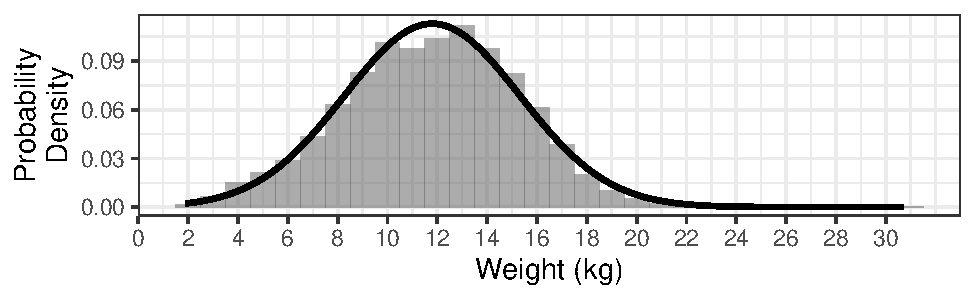
\includegraphics{bookdown-demo_files/figure-latex/unnamed-chunk-23-1.pdf}

\hypertarget{review---the-normal-probability-density-function-pdf}{%
\section{Review - the Normal probability density function (PDF)}\label{review---the-normal-probability-density-function-pdf}}

\[ f(x) = \frac{1}{\sqrt{2\pi\sigma^2}} e^{-\frac{(x-\mu)^2}{2\sigma^2}} \]

\hypertarget{a-simple-model}{%
\section{A simple model}\label{a-simple-model}}

The distribution of weights looks quite unimodal and symmetric, so we will model it with a normal distribution with mean 11.8 and standard deviation 3.53 (N( \(\mu=\) 11.8, \(\sigma=\) 3.53), black line).

\hypertarget{using-the-model-to-make-predictions}{%
\section{Using the Model to Make Predictions}\label{using-the-model-to-make-predictions}}

If you had to predict the weight of one child from this population, what weight would you guess?
\vspace{0.05in}

Is it more likely for a child in Dakar to weigh 10kg, or 20kg? How much more likely?

What is the \emph{probability} of a child in Dakar weighing 11.5 kg?

\hypertarget{likelihood-to-the-rescue}{%
\section{Likelihood to the Rescue!}\label{likelihood-to-the-rescue}}

Which is more likely: three children who weigh 11, 8.2, and 13kg, or three who weigh 10, 12.5 and 15 kg?

How did you:

\begin{itemize}
\tightlist
\item
  Find the likelihood of each observation?
\end{itemize}

\begin{itemize}
\tightlist
\item
  Combine the likelihoods of a set of three observations?
\end{itemize}

What did you have to assume about the set of observations?

\hypertarget{how-does-this-relate-to-linear-regression}{%
\section{How does this relate to linear regression?}\label{how-does-this-relate-to-linear-regression}}

What if we think of this situation as a linear regression problem (with no predictors)?

\begin{Shaded}
\begin{Highlighting}[]
\NormalTok{lm_version <-}\StringTok{ }\KeywordTok{lm}\NormalTok{(AN3 }\OperatorTok{~}\StringTok{ }\DecValTok{1}\NormalTok{, }\DataTypeTok{data =}\NormalTok{ wt)}
\KeywordTok{summary}\NormalTok{(lm_version)}
\end{Highlighting}
\end{Shaded}

\begin{verbatim}
## 
## Call:
## lm(formula = AN3 ~ 1, data = wt)
## 
## Residuals:
## <Labelled double>: Poids de l'enfant (kilogrammes)
##     Min      1Q  Median      3Q     Max 
## -9.8964 -2.3964  0.1036  2.4036 18.9036 
## 
## Labels:
##  value            label
##   99.9 poids non mesuré
## 
## Coefficients:
##             Estimate Std. Error t value Pr(>|t|)    
## (Intercept) 11.79644    0.05435   217.1   <2e-16 ***
## ---
## Signif. codes:  0 '***' 0.001 '**' 0.01 '*' 0.05 '.' 0.1 ' ' 1
## 
## Residual standard error: 3.529 on 4216 degrees of freedom
##   (235 observations deleted due to missingness)
\end{verbatim}

\hypertarget{model-equation}{%
\subsection{Model Equation:}\label{model-equation}}

\hypertarget{likelihood-of-a-dataset-given-a-model}{%
\section{Likelihood of a dataset, given a model}\label{likelihood-of-a-dataset-given-a-model}}

Finally, now, we can understand what we were computing when we did

\begin{Shaded}
\begin{Highlighting}[]
\KeywordTok{logLik}\NormalTok{(lm_version)}
\end{Highlighting}
\end{Shaded}

\begin{verbatim}
## 'log Lik.' -11301.19 (df=2)
\end{verbatim}

For our chosen regression model, we know that the residuals should have a normal distribution with mean 0 and standard deviation \(\sigma\) (estimated Residual Standard Error from R \texttt{summary()} output).

For each data point in the dataset, for a given regression model, we can compute a model prediction.

We can subtract the prediction from the observed response-variable values to get the residuals.

We can compute the \textbf{likelihood} (\(L\)) of this set of residuals by finding the likelihood of each individual residual \(e_i\) in a \(N(0, \sigma)\) distribution.

To get the likelihood of the full dataset given the model, we use the fact that the residuals are independent (they better be, because that was one of the conditions of of linear regression model) -- we can multiply the likelihoods of all the individual residuals together to get the joint likelihood of the full set.

\emph{That} is the ``likelihood'' that is used in the AIC and BIC calculations we considered earlier.

\hypertarget{pdfs-and-pmfs}{%
\chapter{PDFs and PMFs}\label{pdfs-and-pmfs}}

\hypertarget{beyond-normal}{%
\section{Beyond Normal}\label{beyond-normal}}

In our exploration of likelihoods, we did a little bit of work with the Normal probability density function. Here, we will state some characteristics of the normal distribution slightly more formally, and then we will get familiar with some other probability distributions (a.k.a. ``the normal distribution's wierd friends'').

\hypertarget{types-of-probability-distributions}{%
\section{Types of probability distributions}\label{types-of-probability-distributions}}

\hypertarget{continuous-distributions}{%
\subsection{Continuous distributions}\label{continuous-distributions}}

The probability distribution of a continuous variable (one that can take on continuous real values, at least within a certain range) is called a \emph{probability density function} or \textbf{PDF} for short.

PDFs are functions of one continuous variable (we'll call it \(x\)) that have two properties in common:

\begin{itemize}
\tightlist
\item
  The total area under the curve is 1 (\(\int_{-\infty}^{\infty} f(x)dx = 1\))
\item
  The values of the function are non-negative (0, or a positive real number) for all real \(x\) (\(f(x) \geq 0 \forall x \in \mathbb{R}\))
\end{itemize}

For PDFs, the function values (\(y\)-axis values) are \emph{probability densities}, useful for computing likelihoods; probabilities are given by finding \emph{areas} under the curve.

\hypertarget{discrete-distributions}{%
\subsection{Discrete Distributions}\label{discrete-distributions}}

We use categorical as well as quantitative variables in our regression models, so it will prove useful to have some discrete probability distributions as well as continuous ones. Discrete distributions associate each possible value of a discrete variable with its probability of occurence.

A discrete probability distribution is characterized by a \emph{probability mass function} or PMF for short (this is the discrete equivalent of a PDF).

A PMF is a function of one \emph{discrete} variable (we'll call it \(x\)) that have two properties in common:

\begin{itemize}
\tightlist
\item
  The sum of all the function's values is 1 (\(\sum_{x \in S} f(x) =1\), where \(S\) is the set of all possible values \(x\) can have)
\item
  All values of the function are between 0 and 1 inclusive (they are probabilities) (\(f(x) \in [0,1] \forall x \in S\))
\end{itemize}

\hypertarget{relevant-features-of-distributions}{%
\section{Relevant Features of Distributions}\label{relevant-features-of-distributions}}

For this course, the most important features to note about each probability distribuiton will be:

\begin{itemize}
\tightlist
\item
  The \textbf{type} of distribution: discrete or continuous?
\item
  The \textbf{support} of the distribution: what range of possible values can the random variable \(X\) take on?
\item
  The \textbf{parameters} of the distribution. Changing the parameters tunes the center and shape of the distribution, so these are what we need to estimate to fit a particular kind of distribution to a specific dataset. (For example, the parameters of the normal distribution are the mean \(\mu\) and the standard deviation \(\sigma\).)
\item
  The \textbf{shape} of the distribution: what shapes can the function take one? (For example, the normal distribution is always unimodal and symmetric.)
\item
  The PDF or PMF of the distribution. What mathematical expression controls the shape of the distribution?
\item
  We will also note a few examples of variables that might be well modelled by each distribution.
\end{itemize}

\hypertarget{examples-of-continuous-distributions}{%
\section{Examples of Continuous Distributions}\label{examples-of-continuous-distributions}}

\hypertarget{normal}{%
\subsection{Normal}\label{normal}}

\hypertarget{type}{%
\paragraph{Type}\label{type}}

Continuous

\hypertarget{support}{%
\paragraph{Support}\label{support}}

All real numbers

\hypertarget{parameters}{%
\paragraph{Parameters}\label{parameters}}

\begin{itemize}
\tightlist
\item
  \(\mu\), the mean, which can take on any real value
\item
  \(\sigma\), the standard deviation, which can take on any positive real value
\end{itemize}

\hypertarget{shapes}{%
\paragraph{Shapes}\label{shapes}}

The shape is always unimodal and symmetric.

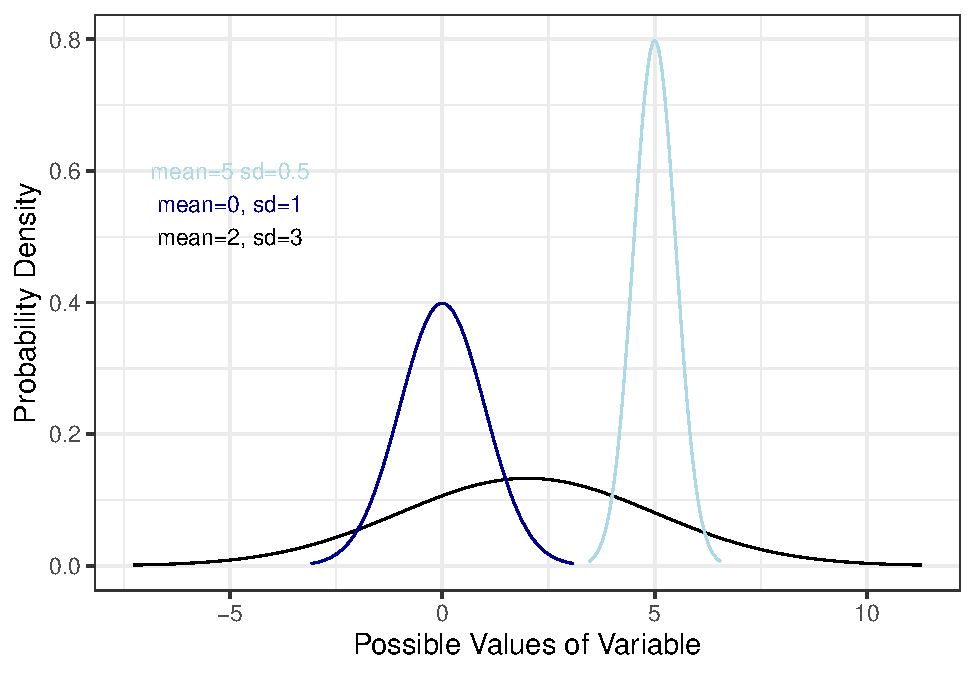
\includegraphics{bookdown-demo_files/figure-latex/unnamed-chunk-26-1.pdf}

\hypertarget{pdf-or-pmf}{%
\paragraph{PDF or PMF}\label{pdf-or-pmf}}

The normal distribution has PDF:

\[ f(x) = \frac{1}{\sqrt{2\pi\sigma^2}}e^{\frac{(x-\mu)^2}{2\sigma^2}}\]

\hypertarget{examples}{%
\paragraph{Examples}\label{examples}}

A normal distribution might be a good fit for data on childrens' weights in kg, or for the duration of visits at a zoo, or\ldots{}

\hypertarget{gamma}{%
\subsection{Gamma}\label{gamma}}

\hypertarget{type-1}{%
\paragraph{Type}\label{type-1}}

Continuous

\hypertarget{support-1}{%
\paragraph{Support}\label{support-1}}

positive real numbers

\hypertarget{parameters-1}{%
\paragraph{Parameters}\label{parameters-1}}

There are two alternate but equivalent parameterizations for the gamma distribution.

The first option: \(\alpha\) (shape) and \(\beta\) (rate), where \(\alpha>0\) and \(\beta>0\)

The second option: \(k\) (shape) and \(\theta\) (scale), where \(k >0\) and \(\theta>0\).

Converting between the two parameterizations: \(\alpha = k\) and \(\beta = \frac{1}{\theta}\).

\hypertarget{shapes-1}{%
\paragraph{Shapes}\label{shapes-1}}

The gamma distribution can take on a unimodal, symmetric shape or a unimodal shape with any amount of right skew (up to an exponential distribution shape).

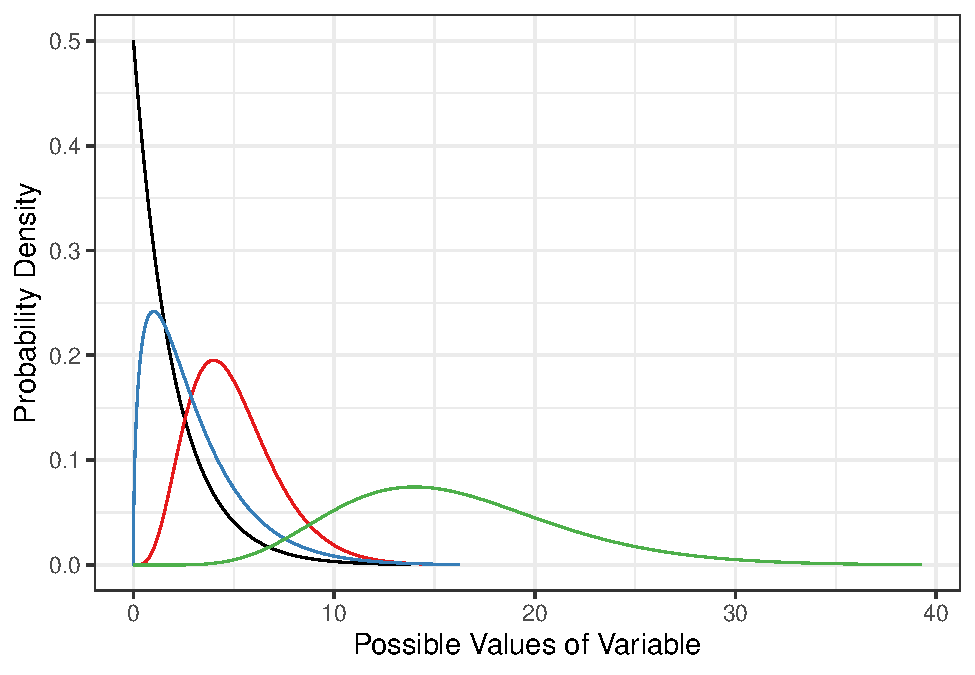
\includegraphics{bookdown-demo_files/figure-latex/unnamed-chunk-27-1.pdf}

Note: you don't need to be familiar with exactly how the different values of parameters influence the shape of the gamma distribution PDF, so the curves here are not labelled with parameter values.

\hypertarget{pdf-or-pmf-1}{%
\paragraph{PDF or PMF}\label{pdf-or-pmf-1}}

The gamma distribution has PDF:

\[ f(x) = \frac{1}{\Gamma(k) \theta^k}x^{(k-1)}e^{\frac{-x}{\theta}}\]
Where \(\Gamma\) is the Gamma function (look up the definition if you choose),
or equivalently,

\[ f(x) = \frac{\beta^{\alpha}}{\Gamma(\alpha)}x^{(\alpha-1)}e^{-\beta x}\]

\hypertarget{examples-1}{%
\paragraph{Examples}\label{examples-1}}

Gamma distributions are often used to model things like wind speed or duration of an event (any quantity that might have right skew and is never negative).

\hypertarget{beta}{%
\subsection{Beta}\label{beta}}

\hypertarget{type-2}{%
\paragraph{Type}\label{type-2}}

Continuous

\hypertarget{support-2}{%
\paragraph{Support}\label{support-2}}

Real numbers between 0 and 1 ({[}0,1{]})

\hypertarget{parameters-2}{%
\paragraph{Parameters}\label{parameters-2}}

\(\alpha\) (shape 1) and \(\beta\) (shape 2), both of which must be \(>1\).

\hypertarget{shapes-2}{%
\paragraph{Shapes}\label{shapes-2}}

This distribution can take on almost any shape, for example:

\begin{Shaded}
\begin{Highlighting}[]
\KeywordTok{gf_dist}\NormalTok{(}\StringTok{'beta'}\NormalTok{, }\DataTypeTok{params =} \KeywordTok{c}\NormalTok{(}\DataTypeTok{shape1=}\DecValTok{5}\NormalTok{, }\DataTypeTok{shape2=}\DecValTok{1}\NormalTok{)) }\OperatorTok
\StringTok{  }\KeywordTok{gf_dist}\NormalTok{(}\StringTok{'beta'}\NormalTok{, }\DataTypeTok{params =} \KeywordTok{c}\NormalTok{(}\DataTypeTok{shape1=}\DecValTok{1}\NormalTok{, }\DataTypeTok{shape2=}\DecValTok{3}\NormalTok{), }\DataTypeTok{color=}\NormalTok{colrs[}\DecValTok{1}\NormalTok{]) }\OperatorTok
\StringTok{  }\KeywordTok{gf_dist}\NormalTok{(}\StringTok{'beta'}\NormalTok{, }\DataTypeTok{params =} \KeywordTok{c}\NormalTok{(}\DataTypeTok{shape1=}\DecValTok{2}\NormalTok{, }\DataTypeTok{shape2=}\DecValTok{2}\NormalTok{), }\DataTypeTok{color=}\NormalTok{colrs[}\DecValTok{2}\NormalTok{]) }\OperatorTok
\StringTok{  }\KeywordTok{gf_dist}\NormalTok{(}\StringTok{'beta'}\NormalTok{, }\DataTypeTok{params =} \KeywordTok{c}\NormalTok{(}\DataTypeTok{shape1=}\DecValTok{2}\NormalTok{, }\DataTypeTok{shape2=}\DecValTok{5}\NormalTok{), }\DataTypeTok{color=}\NormalTok{colrs[}\DecValTok{3}\NormalTok{]) }\OperatorTok
\StringTok{  }\KeywordTok{gf_dist}\NormalTok{(}\StringTok{'beta'}\NormalTok{, }\DataTypeTok{params =} \KeywordTok{c}\NormalTok{(}\DataTypeTok{shape1=}\FloatTok{0.5}\NormalTok{, }\DataTypeTok{shape2=}\FloatTok{0.5}\NormalTok{), }\DataTypeTok{color=}\NormalTok{colrs[}\DecValTok{4}\NormalTok{]) }\OperatorTok
\StringTok{  }\KeywordTok{gf_labs}\NormalTok{(}\DataTypeTok{x=}\StringTok{'Possible Values of Variable'}\NormalTok{, }\DataTypeTok{y=}\StringTok{'Probability Density'}\NormalTok{) }\OperatorTok
\StringTok{  }\KeywordTok{gf_lims}\NormalTok{(}\DataTypeTok{y=}\KeywordTok{c}\NormalTok{(}\DecValTok{0}\NormalTok{,}\FloatTok{2.5}\NormalTok{))}
\end{Highlighting}
\end{Shaded}

\begin{verbatim}
## Warning: Removed 796 rows containing missing values (geom_path).
\end{verbatim}

\begin{verbatim}
## Warning: Removed 436 rows containing missing values (geom_path).
\end{verbatim}

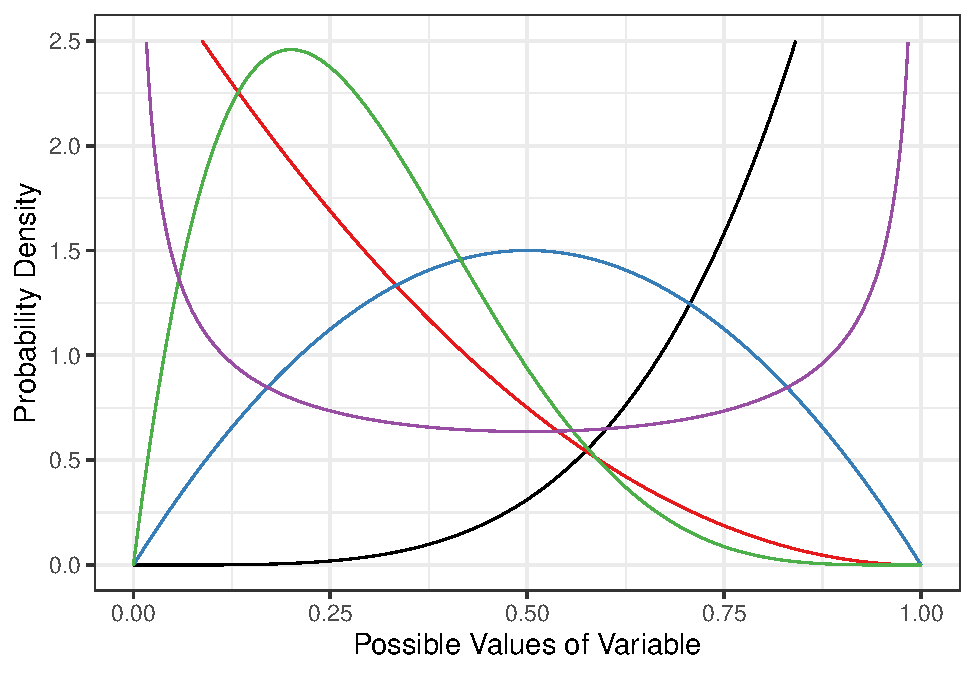
\includegraphics{bookdown-demo_files/figure-latex/unnamed-chunk-28-1.pdf}

\hypertarget{pdf-or-pmf-2}{%
\paragraph{PDF or PMF}\label{pdf-or-pmf-2}}

The PDF is:

\[ f(x) = \frac{x^{(\alpha -1)}(1-x)^{(\beta-1)}}{ B(\alpha, \beta)}\]
Where \(B\) is the Beta function (again, feel free to look up the definition if you are interested).

\hypertarget{examples-2}{%
\paragraph{Examples}\label{examples-2}}

Beta distributions could be used for any variable that takes on values between 0-1, for example, baseball players' batting averages, or test scores (as proportions).

\hypertarget{examples-of-discrete-distributions}{%
\section{Examples of Discrete Distributions}\label{examples-of-discrete-distributions}}

\hypertarget{binomial}{%
\subsection{Binomial}\label{binomial}}

\hypertarget{type-3}{%
\paragraph{Type}\label{type-3}}

Discrete

\hypertarget{support-3}{%
\paragraph{Support}\label{support-3}}

You can think about the support of this distribution two ways.
Technically, the support is \(k= 0, 1,2,3,\dots\): 0 and positive integers, interpreted as the number of ``successes'' in \(n\) binomial trials. Binomial trials are independent observations of a process that has two possible outcomes, ``success'' or ``failure'', with set probabilities of each occurring. (And probabilities of success and failure must sum to 1.)

So, for each individual binomial trial, the possible outcomes are 0 and 1, often interpreted as TRUE and FALSE or ``success'' and ``failure''.

For our purposes, this distribution will be useful for modelling response variables that are categorical with two possible values (and the \(n\) trials will be the \(n\) rows in our dataset).

\hypertarget{parameters-3}{%
\paragraph{Parameters}\label{parameters-3}}

Parameters are \(n\), the number of independent trials, and \(p\), the probability of success in each trial.

\hypertarget{shapes-3}{%
\paragraph{Shapes}\label{shapes-3}}

The figure below shows the shape of binomial distributions with fixed \(n=100\) and varying \(p\):

\begin{Shaded}
\begin{Highlighting}[]
\KeywordTok{gf_dist}\NormalTok{(}\StringTok{'binom'}\NormalTok{, }\DataTypeTok{params =} \KeywordTok{c}\NormalTok{(}\DataTypeTok{size=}\DecValTok{100}\NormalTok{, }\DataTypeTok{prob=}\FloatTok{0.1}\NormalTok{), }\DataTypeTok{color=}\NormalTok{colrs[}\DecValTok{1}\NormalTok{]) }\OperatorTok
\StringTok{  }\KeywordTok{gf_dist}\NormalTok{(}\StringTok{'binom'}\NormalTok{, }\DataTypeTok{params =} \KeywordTok{c}\NormalTok{(}\DataTypeTok{size=}\DecValTok{100}\NormalTok{, }\DataTypeTok{prob=}\FloatTok{0.25}\NormalTok{), }\DataTypeTok{color=}\NormalTok{colrs[}\DecValTok{2}\NormalTok{]) }\OperatorTok
\StringTok{  }\KeywordTok{gf_dist}\NormalTok{(}\StringTok{'binom'}\NormalTok{, }\DataTypeTok{params =} \KeywordTok{c}\NormalTok{(}\DataTypeTok{size=}\DecValTok{100}\NormalTok{, }\DataTypeTok{prob=}\FloatTok{0.5}\NormalTok{), }\DataTypeTok{color=}\NormalTok{colrs[}\DecValTok{3}\NormalTok{]) }\OperatorTok
\StringTok{  }\KeywordTok{gf_dist}\NormalTok{(}\StringTok{'binom'}\NormalTok{, }\DataTypeTok{params =} \KeywordTok{c}\NormalTok{(}\DataTypeTok{size=}\DecValTok{100}\NormalTok{, }\DataTypeTok{prob=}\FloatTok{0.75}\NormalTok{), }\DataTypeTok{color=}\NormalTok{colrs[}\DecValTok{4}\NormalTok{]) }\OperatorTok
\StringTok{  }\KeywordTok{gf_dist}\NormalTok{(}\StringTok{'binom'}\NormalTok{, }\DataTypeTok{params =} \KeywordTok{c}\NormalTok{(}\DataTypeTok{size=}\DecValTok{100}\NormalTok{, }\DataTypeTok{prob=}\FloatTok{0.99}\NormalTok{), }\DataTypeTok{color=}\NormalTok{colrs[}\DecValTok{5}\NormalTok{]) }\OperatorTok
\StringTok{  }\KeywordTok{gf_labs}\NormalTok{(}\DataTypeTok{x=}\StringTok{'k, the Number of Successes in 100 Trials'}\NormalTok{, }\DataTypeTok{y=}\StringTok{'Probability'}\NormalTok{)}
\end{Highlighting}
\end{Shaded}

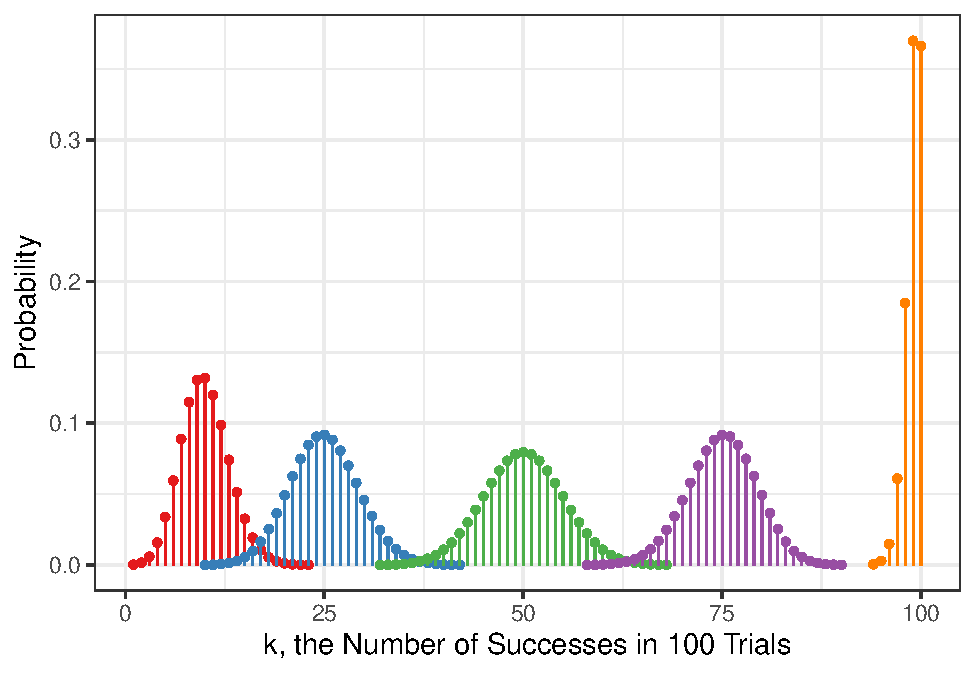
\includegraphics{bookdown-demo_files/figure-latex/unnamed-chunk-29-1.pdf}

The \(p\) used were 0.1, 0.25, 0.5, 0.75, and 0.99. Can you tell which is which?

\hypertarget{pdf-or-pmf-3}{%
\paragraph{PDF or PMF}\label{pdf-or-pmf-3}}

The PMF for the binomial distribution is:
\[ P(X=k \vert n,p) = {n \choose k} p^k (1-p)^{n-k}\]

Where \(k\) is the number of successes observed in \(n\) trials (you can think of \(k\) as our ``x-axis variable'' for this PMF).

\hypertarget{examples-3}{%
\paragraph{Examples}\label{examples-3}}

We might use this distribution to model any categorical variable with two possible values, like Age (if possible values are ``adult'' and ``child'') or health status (``has disease'' or ``does not have disease''). We'll think of each observation in the dataset as one of the \(n\) indpendent trials, with one of two possible outcomes for each trial.

\hypertarget{poisson}{%
\subsection{Poisson}\label{poisson}}

\hypertarget{type-4}{%
\paragraph{Type}\label{type-4}}

Discrete

\hypertarget{support-4}{%
\paragraph{Support}\label{support-4}}

The support is 0 and positive integers (i.e., this distribution works well for count data).

\hypertarget{parameters-4}{%
\paragraph{Parameters}\label{parameters-4}}

The Poisson distribution has one parameter, \(\lambda\) (the event rate per unit time) which must be greater than 0.

\hypertarget{shapes-4}{%
\paragraph{Shapes}\label{shapes-4}}

The distribution can take on unimodal shapes with varying amounts of right skew (from none, to an exponential shape).

\begin{Shaded}
\begin{Highlighting}[]
\NormalTok{colrs <-}\StringTok{ }\NormalTok{RColorBrewer}\OperatorTok{::}\KeywordTok{brewer.pal}\NormalTok{(}\DecValTok{8}\NormalTok{, }\StringTok{'Set2'}\NormalTok{)}
\KeywordTok{gf_dist}\NormalTok{(}\StringTok{'pois'}\NormalTok{, }\DataTypeTok{params=}\KeywordTok{c}\NormalTok{(}\DataTypeTok{lambda=}\FloatTok{0.5}\NormalTok{), }\DataTypeTok{color=}\NormalTok{colrs[}\DecValTok{1}\NormalTok{]) }\OperatorTok
\StringTok{  }\KeywordTok{gf_dist}\NormalTok{(}\StringTok{'pois'}\NormalTok{, }\DataTypeTok{params=}\KeywordTok{c}\NormalTok{(}\DataTypeTok{lambda=}\DecValTok{3}\NormalTok{), }\DataTypeTok{color=}\NormalTok{colrs[}\DecValTok{2}\NormalTok{]) }\OperatorTok
\StringTok{  }\KeywordTok{gf_dist}\NormalTok{(}\StringTok{'pois'}\NormalTok{, }\DataTypeTok{params=}\KeywordTok{c}\NormalTok{(}\DataTypeTok{lambda=}\DecValTok{6}\NormalTok{), }\DataTypeTok{color=}\NormalTok{colrs[}\DecValTok{3}\NormalTok{]) }\OperatorTok
\StringTok{  }\KeywordTok{gf_dist}\NormalTok{(}\StringTok{'pois'}\NormalTok{, }\DataTypeTok{params=}\KeywordTok{c}\NormalTok{(}\DataTypeTok{lambda=}\DecValTok{15}\NormalTok{), }\DataTypeTok{color=}\NormalTok{colrs[}\DecValTok{4}\NormalTok{]) }\OperatorTok
\StringTok{  }\KeywordTok{gf_labs}\NormalTok{(}\DataTypeTok{x=}\StringTok{'k (number of events)'}\NormalTok{, }\DataTypeTok{y=}\StringTok{'Probability'}\NormalTok{)}
\end{Highlighting}
\end{Shaded}

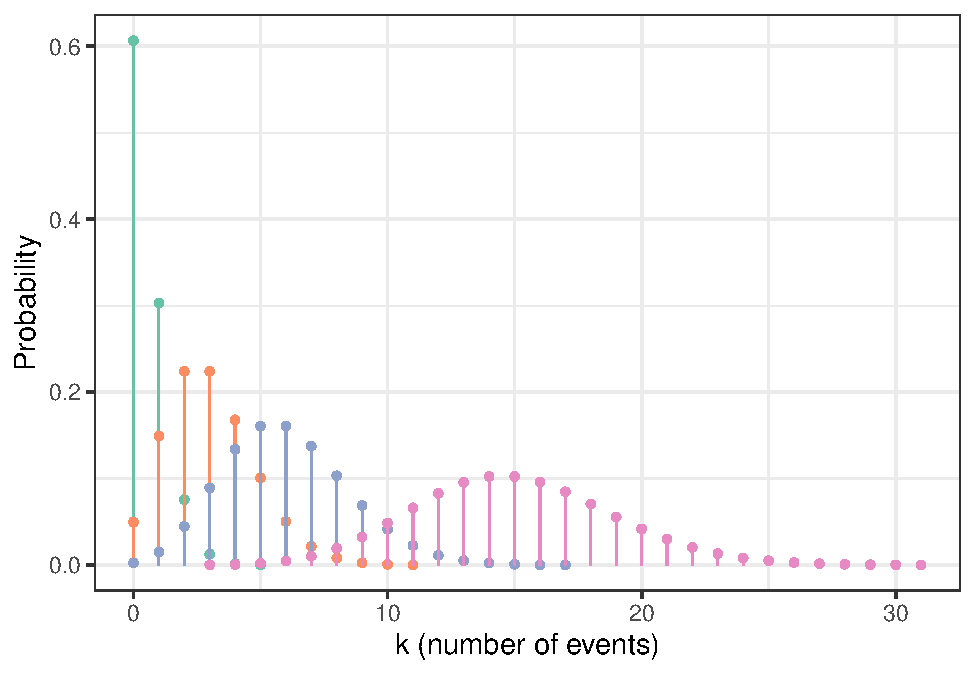
\includegraphics{bookdown-demo_files/figure-latex/unnamed-chunk-30-1.pdf}

\hypertarget{pdf-or-pmf-4}{%
\paragraph{PDF or PMF}\label{pdf-or-pmf-4}}

The Poisson PMF is:

\[P(X=k \vert \lambda) = \frac{\lambda^k e^{-\lambda}}{k!}\]

\hypertarget{examples-4}{%
\paragraph{Examples}\label{examples-4}}

The Poisson distribution might be used to model any response variable that is comprised of counts, for example, the number of birds sighted in a bird survey, or the number of people admitted to an emergency room each hour.

\hypertarget{negative-binomial}{%
\subsection{Negative Binomial}\label{negative-binomial}}

There are two versions or ``types'' of this distribution, cleverly known as NB1 (type 1) and NB2 (type 2). NB1 has ``constant overdispersion'' -- the variance of the distribution is greater than the mean according to a constant ratio. NB2 has ``variable overdispersion'' -- the variance is a quadratic function of the mean. The NB2 is the one that corresponds directly to conceptualization in terms of binomial trials (with the PMF giving the probability of observing \(y\) failures before the \(r\)th success). \href{https://www.amazon.com/Generalized-Linear-Models-Extensions-Third/dp/1597181056/ref=sr_1_1?s=books\&ie=UTF8\&qid=1538705158\&sr=1-1\&keywords=Generalized+Linear+Models+and+Extensions\%3A+third+edition}{Hardin and Hilbe 2007} describe the negative binomial this way: ``Instead of counts entering uniformly, we see counts entering with a specific gamma-distributed shape.''

\hypertarget{type-5}{%
\paragraph{Type}\label{type-5}}

Discrete

\hypertarget{support-5}{%
\paragraph{Support}\label{support-5}}

The support is 0 and positive integers (i.e., this distribution works well for count data). It also has a derivation in terms of binomial trials, but in our regression models, we will only use it with count data.

\hypertarget{parameters-5}{%
\paragraph{Parameters}\label{parameters-5}}

A common parameterization of the negative binomial (online and in actuarial science) has parameters \(p\), the probability of success on each binomial trial, and \(r\), the number of failures observed. The PMF then gives the probability of observing \(k\) failures before the \(r\)th success in a series of Bernoulli trials.

Here, we will use an alternate parameterization. The other common way to parameterize and derive the NB is as a Poisson-gamma mixture -- a modified version of a Poisson distribution. In this scheme, the parameters of the distribution are \(\mu\) and \(\alpha\).

\hypertarget{shapes-5}{%
\paragraph{Shapes}\label{shapes-5}}

These distributions can take on unimodal shapes with varying amounts of right skew. In NB2 (type 2) distributions the variance (spread) is larger relative to the mean.

NB1:

\begin{Shaded}
\begin{Highlighting}[]
\KeywordTok{require}\NormalTok{(gamlss.dist)}
\NormalTok{colrs <-}\StringTok{ }\NormalTok{RColorBrewer}\OperatorTok{::}\KeywordTok{brewer.pal}\NormalTok{(}\DecValTok{8}\NormalTok{, }\StringTok{'Set2'}\NormalTok{)}
\KeywordTok{gf_dist}\NormalTok{(}\StringTok{'NBI'}\NormalTok{, }\DataTypeTok{params=}\KeywordTok{c}\NormalTok{(}\DataTypeTok{mu=}\DecValTok{1}\NormalTok{, }\DataTypeTok{sigma=}\FloatTok{0.5}\NormalTok{), }\DataTypeTok{color=}\NormalTok{colrs[}\DecValTok{1}\NormalTok{]) }\OperatorTok
\StringTok{  }\KeywordTok{gf_dist}\NormalTok{(}\StringTok{'NBI'}\NormalTok{, }\DataTypeTok{params=}\KeywordTok{c}\NormalTok{(}\DataTypeTok{mu=}\DecValTok{1}\NormalTok{, }\DataTypeTok{sigma=}\FloatTok{0.5}\NormalTok{), }\DataTypeTok{color=}\NormalTok{colrs[}\DecValTok{2}\NormalTok{]) }\OperatorTok
\StringTok{  }\KeywordTok{gf_dist}\NormalTok{(}\StringTok{'NBI'}\NormalTok{, }\DataTypeTok{params=}\KeywordTok{c}\NormalTok{(}\DataTypeTok{mu=}\DecValTok{4}\NormalTok{, }\DataTypeTok{sigma=}\DecValTok{1}\NormalTok{), }\DataTypeTok{color=}\NormalTok{colrs[}\DecValTok{3}\NormalTok{]) }\OperatorTok
\StringTok{  }\KeywordTok{gf_dist}\NormalTok{(}\StringTok{'NBI'}\NormalTok{, }\DataTypeTok{params=}\KeywordTok{c}\NormalTok{(}\DataTypeTok{mu=}\DecValTok{15}\NormalTok{, }\DataTypeTok{sigma=}\DecValTok{4}\NormalTok{), }\DataTypeTok{color=}\NormalTok{colrs[}\DecValTok{4}\NormalTok{]) }\OperatorTok
\StringTok{  }\KeywordTok{gf_lims}\NormalTok{(}\DataTypeTok{x=}\KeywordTok{c}\NormalTok{(}\DecValTok{0}\NormalTok{,}\DecValTok{20}\NormalTok{)) }\OperatorTok
\StringTok{  }\KeywordTok{gf_labs}\NormalTok{(}\DataTypeTok{x=}\StringTok{'k (number of events)'}\NormalTok{, }\DataTypeTok{y=}\StringTok{'Probability'}\NormalTok{)}
\end{Highlighting}
\end{Shaded}

\begin{verbatim}
## Warning: Removed 15 rows containing missing values (geom_segment).
\end{verbatim}

\begin{verbatim}
## Warning: Removed 15 rows containing missing values (geom_point).
\end{verbatim}

\begin{verbatim}
## Warning: Removed 177 rows containing missing values (geom_segment).
\end{verbatim}

\begin{verbatim}
## Warning: Removed 177 rows containing missing values (geom_point).
\end{verbatim}

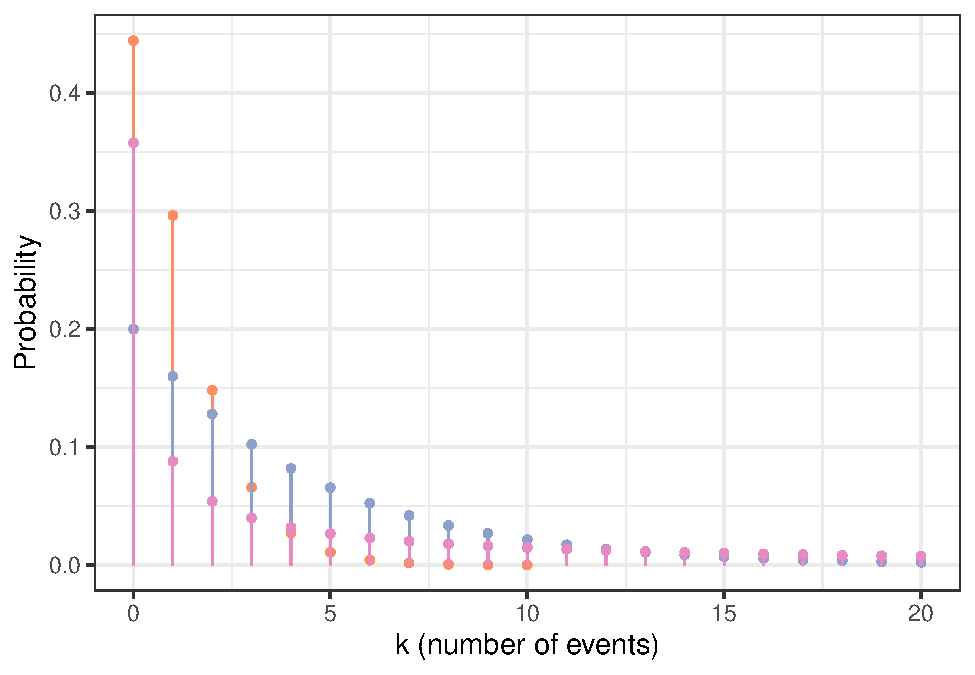
\includegraphics{bookdown-demo_files/figure-latex/unnamed-chunk-31-1.pdf}

NB2:

\begin{Shaded}
\begin{Highlighting}[]
\NormalTok{colrs <-}\StringTok{ }\NormalTok{RColorBrewer}\OperatorTok{::}\KeywordTok{brewer.pal}\NormalTok{(}\DecValTok{8}\NormalTok{, }\StringTok{'Set2'}\NormalTok{)}
\KeywordTok{gf_dist}\NormalTok{(}\StringTok{'NBII'}\NormalTok{, }\DataTypeTok{params=}\KeywordTok{c}\NormalTok{(}\DataTypeTok{mu=}\DecValTok{1}\NormalTok{, }\DataTypeTok{sigma=}\FloatTok{0.5}\NormalTok{), }\DataTypeTok{color=}\NormalTok{colrs[}\DecValTok{1}\NormalTok{]) }\OperatorTok
\StringTok{  }\KeywordTok{gf_dist}\NormalTok{(}\StringTok{'NBII'}\NormalTok{, }\DataTypeTok{params=}\KeywordTok{c}\NormalTok{(}\DataTypeTok{mu=}\DecValTok{1}\NormalTok{, }\DataTypeTok{sigma=}\FloatTok{0.5}\NormalTok{), }\DataTypeTok{color=}\NormalTok{colrs[}\DecValTok{2}\NormalTok{]) }\OperatorTok
\StringTok{  }\KeywordTok{gf_dist}\NormalTok{(}\StringTok{'NBII'}\NormalTok{, }\DataTypeTok{params=}\KeywordTok{c}\NormalTok{(}\DataTypeTok{mu=}\DecValTok{4}\NormalTok{, }\DataTypeTok{sigma=}\DecValTok{1}\NormalTok{), }\DataTypeTok{color=}\NormalTok{colrs[}\DecValTok{3}\NormalTok{]) }\OperatorTok
\StringTok{  }\KeywordTok{gf_dist}\NormalTok{(}\StringTok{'NBII'}\NormalTok{, }\DataTypeTok{params=}\KeywordTok{c}\NormalTok{(}\DataTypeTok{mu=}\DecValTok{15}\NormalTok{, }\DataTypeTok{sigma=}\DecValTok{4}\NormalTok{), }\DataTypeTok{color=}\NormalTok{colrs[}\DecValTok{4}\NormalTok{]) }\OperatorTok
\StringTok{  }\KeywordTok{gf_lims}\NormalTok{(}\DataTypeTok{x=}\KeywordTok{c}\NormalTok{(}\DecValTok{0}\NormalTok{,}\DecValTok{20}\NormalTok{)) }\OperatorTok
\StringTok{  }\KeywordTok{gf_labs}\NormalTok{(}\DataTypeTok{x=}\StringTok{'k (number of events)'}\NormalTok{, }\DataTypeTok{y=}\StringTok{'Probability'}\NormalTok{)}
\end{Highlighting}
\end{Shaded}

\begin{verbatim}
## Warning: Removed 1 rows containing missing values (geom_segment).
\end{verbatim}

\begin{verbatim}
## Warning: Removed 1 rows containing missing values (geom_point).
\end{verbatim}

\begin{verbatim}
## Warning: Removed 39 rows containing missing values (geom_segment).
\end{verbatim}

\begin{verbatim}
## Warning: Removed 39 rows containing missing values (geom_point).
\end{verbatim}

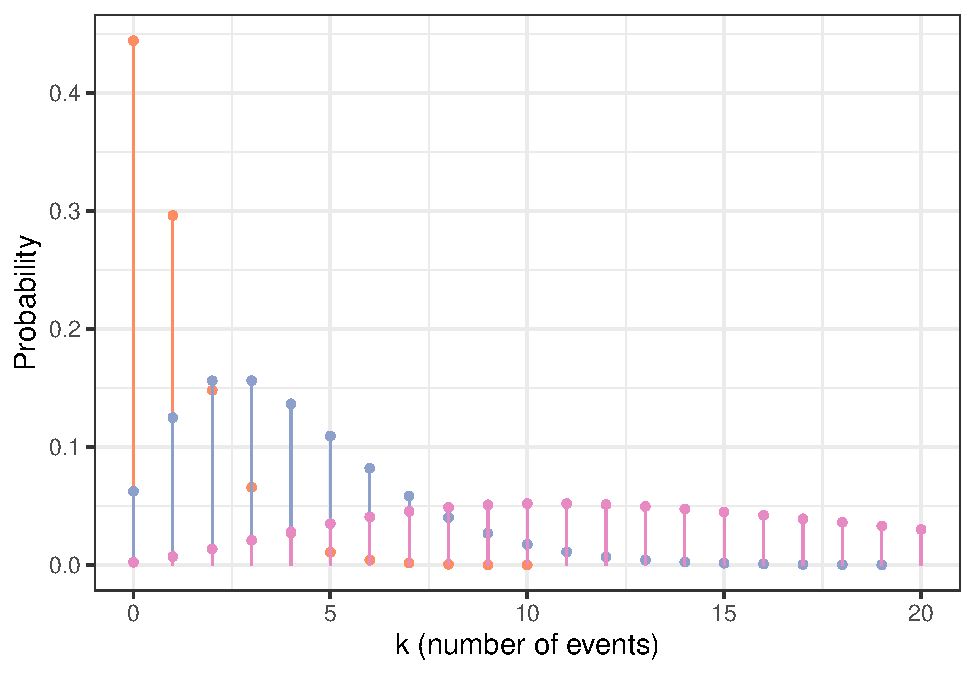
\includegraphics{bookdown-demo_files/figure-latex/unnamed-chunk-32-1.pdf}

\hypertarget{pdf-or-pmf-5}{%
\paragraph{PDF or PMF}\label{pdf-or-pmf-5}}

Details of the parameterizations and likelihood and fitting of NB1 and NB2 distributions can be found in \href{https://www.amazon.com/Generalized-Linear-Models-Extensions-Third/dp/1597181056/ref=sr_1_1?s=books\&ie=UTF8\&qid=1538705158\&sr=1-1\&keywords=Generalized+Linear+Models+and+Extensions\%3A+third+edition}{Hardin and Hilbe 2007}, if you are interested.

The PMF for the NB1, where the variance is a constant multiple of the mean, is:

\[ f(x \vert \mu, \alpha) = \frac{\Gamma(x + \mu)}{\Gamma(\mu)\Gamma(x+1)}(\frac{1}{1+\alpha})^\mu(\frac{\alpha}{1+\alpha})^x \]

Where \(\Gamma\) is a Gamma function. Note that if \(\alpha\) = 0 this becomes a Poisson distribution, so the Poisson is a special case of the NB1.

The PMF for the NB2, where the variance is a quadratic function of the mean, is:

\[ f(x \vert \mu, \alpha) = \frac{\Gamma(x + \frac{1}{\alpha})}{\Gamma(\frac{1}{\alpha})\Gamma(x+1)}(\frac{1}{1+\alpha \mu})^{\frac{1}{\alpha}}(1 - \frac{1}{1+\alpha \mu})^x \]

\hypertarget{examples-5}{%
\paragraph{Examples}\label{examples-5}}

NB distributions are good models for overdispersed count data, where (in the regression context) the residual variance is not equal to the expected (predicted) value. (Note that if you are reading this before learning about regression models for count data, you may not understand this sentence yet\ldots don't worry, it will make sense when you return later!) Some examples might include sightings data on numbers of animals seen on wildlife surveys, or the number of items bought per order at an online retailer.

\hypertarget{a-mixture-distribution-tweedie}{%
\subsection{A Mixture Distribution: Tweedie}\label{a-mixture-distribution-tweedie}}

The Tweedie family of distributions is a very large one - depending on the values of the different parameters, the PMF/PDF can be written in many different ways, and it can take on many different shapes. The description below is a simplified one, geared toward the types of Tweedie distributions we are likely to try to use in regression models in this course -- mainly the ``compound Poisson-gamma'' type.

\emph{Some extra resources for which you will not be held responsible in this course:}

\begin{itemize}
\item
  You can find an accessible description and example of this kind of distribution at: \url{http://www.notenoughthoughts.net/posts/modeling-activity.html}.
\item
  The following site may also be useful in regard to using the Tweedie in regression models: \url{http://support.sas.com/documentation/cdl/en/statug/68162/HTML/default/viewer.htm\#statug_genmod_details28.htm}
\end{itemize}

\hypertarget{type-6}{%
\paragraph{Type}\label{type-6}}

These distributions are \emph{both} continuous and discrete - a kind of mix of a Poisson distribution and gamma distribution(s).

\hypertarget{support-6}{%
\paragraph{Support}\label{support-6}}

The support is non-negative real numbers (greater than or equal to 0).

\hypertarget{parameters-6}{%
\paragraph{Parameters}\label{parameters-6}}

(Note: there are multiple different ways to parameterize these distributions.) We will use:

\begin{itemize}
\tightlist
\item
  \(p\), the index or power parameter, which can be 0 (resulting in a normal distribution), 1 (resulting in a Poisson distribution), \textbf{\(1 < p < 2\) (a compound Poisson-gamma distribution -- what we will mainly use)}, 2 (a gamma distribution), 3 (an inverse Gaussian distribution), \(<3\) (a positive stable distribution), or \(\infty\) (an extreme positive stable distribuiton). For the case where \(1 < p < 2\), and the distribution is a compound of a Poisson and a gamma, then \(p = \frac{k+2}{k+1}\) where \(k\) is the parameter of the gamma distribution. When \(1<p<2\), \(p\) closer to 1 means thant the Poisson distribution (the mass at 0) gets more ``weight'' in the compound distribution, and values of \(p\) closer to 2 mean that the gamma distribution gets more ``weight.''
\item
  \(\mu\). For the case where \(1 < p < 2\), and the distribution is a compound of a Poisson and a gamma, then \(\mu = \lambda k \theta\) where \(\lambda\) is the parameter of the Poisson distribution and \(k\) and \(\theta\) are the parameters of the gamma.
\item
  \(\phi\) For the case where \(1 < p < 2\), and the distribution is a compound of a Poisson and a gamma, then \(\phi = \frac{\lambda^{(1-p)} (k \theta) ^{(2-p)}}{2-p}\) where \(\lambda\) is the parameter of the Poisson distribution and \(k\) and \(\theta\) are the parameters of the gamma.
\end{itemize}

\hypertarget{shapes-6}{%
\paragraph{Shapes}\label{shapes-6}}

A compound Poisson-gamma Tweedie distribution can take on varying shapes; the main characteristic of interest for us is that it can have a mass at 0, then a unimodal or multimodal distribution with a long right tail (lots of right skew).

\begin{Shaded}
\begin{Highlighting}[]
\KeywordTok{require}\NormalTok{(tweedie)}
\NormalTok{tex <-}\StringTok{ }\KeywordTok{data.frame}\NormalTok{(}\DataTypeTok{x=}\KeywordTok{seq}\NormalTok{(}\DataTypeTok{from=}\DecValTok{0}\NormalTok{, }\DataTypeTok{by=}\FloatTok{0.1}\NormalTok{, }\DataTypeTok{to=}\DecValTok{50}\NormalTok{)) }\OperatorTok
\StringTok{  }\KeywordTok{mutate}\NormalTok{(}\DataTypeTok{dens.a =} \KeywordTok{dtweedie}\NormalTok{(x, }\DataTypeTok{xi =} \FloatTok{1.1}\NormalTok{, }\DataTypeTok{mu=}\DecValTok{4}\NormalTok{, }\DataTypeTok{phi=}\DecValTok{2}\NormalTok{)) }\OperatorTok
\StringTok{  }\KeywordTok{mutate}\NormalTok{(}\DataTypeTok{dens.b =} \KeywordTok{dtweedie}\NormalTok{(x, }\DataTypeTok{xi =} \FloatTok{1.3}\NormalTok{, }\DataTypeTok{mu=}\DecValTok{4}\NormalTok{, }\DataTypeTok{phi=}\FloatTok{0.5}\NormalTok{)) }\OperatorTok
\StringTok{  }\KeywordTok{mutate}\NormalTok{(}\DataTypeTok{dens.c =} \KeywordTok{dtweedie}\NormalTok{(x, }\DataTypeTok{xi =} \FloatTok{1.5}\NormalTok{, }\DataTypeTok{mu=}\DecValTok{4}\NormalTok{, }\DataTypeTok{phi=}\FloatTok{0.3}\NormalTok{)) }\OperatorTok
\StringTok{  }\KeywordTok{mutate}\NormalTok{(}\DataTypeTok{dens.d =} \KeywordTok{dtweedie}\NormalTok{(x, }\DataTypeTok{xi =} \FloatTok{1.8}\NormalTok{, }\DataTypeTok{mu=}\DecValTok{4}\NormalTok{, }\DataTypeTok{phi=}\DecValTok{1}\NormalTok{)) }\OperatorTok
\StringTok{  }\KeywordTok{mutate}\NormalTok{(}\DataTypeTok{dens.e =} \KeywordTok{dtweedie}\NormalTok{(x, }\DataTypeTok{xi =} \FloatTok{1.5}\NormalTok{, }\DataTypeTok{mu=}\DecValTok{4}\NormalTok{, }\DataTypeTok{phi=}\DecValTok{5}\NormalTok{))}
  

\KeywordTok{gf_line}\NormalTok{(dens.a }\OperatorTok{~}\StringTok{ }\NormalTok{x, }\DataTypeTok{data=}\NormalTok{tex, }\DataTypeTok{color=}\NormalTok{colrs[}\DecValTok{1}\NormalTok{]) }\OperatorTok
\StringTok{  }\KeywordTok{gf_line}\NormalTok{(dens.b }\OperatorTok{~}\NormalTok{x, }\DataTypeTok{data=}\NormalTok{tex, }\DataTypeTok{color=}\NormalTok{colrs[}\DecValTok{2}\NormalTok{]) }\OperatorTok
\StringTok{  }\KeywordTok{gf_line}\NormalTok{(dens.c }\OperatorTok{~}\NormalTok{x, }\DataTypeTok{data=}\NormalTok{tex, }\DataTypeTok{color=}\NormalTok{colrs[}\DecValTok{3}\NormalTok{]) }\OperatorTok
\StringTok{  }\KeywordTok{gf_line}\NormalTok{(dens.d }\OperatorTok{~}\NormalTok{x, }\DataTypeTok{data=}\NormalTok{tex, }\DataTypeTok{color=}\NormalTok{colrs[}\DecValTok{4}\NormalTok{]) }\OperatorTok
\StringTok{  }\KeywordTok{gf_line}\NormalTok{(dens.e }\OperatorTok{~}\NormalTok{x, }\DataTypeTok{data=}\NormalTok{tex, }\DataTypeTok{color=}\NormalTok{colrs[}\DecValTok{5}\NormalTok{])}
\end{Highlighting}
\end{Shaded}

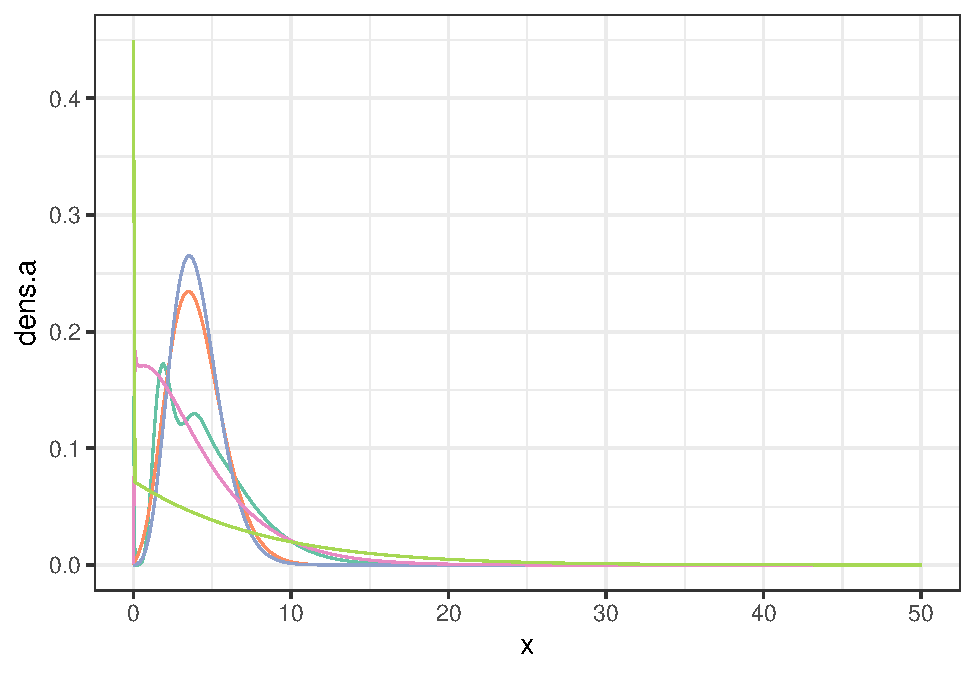
\includegraphics{bookdown-demo_files/figure-latex/unnamed-chunk-33-1.pdf}

\hypertarget{pdf-or-pmf-6}{%
\paragraph{PDF or PMF}\label{pdf-or-pmf-6}}

A Tweedie distribution with \(p>1\) has the form:

\[ f(X \vert \mu, \phi, p) = a(x, \phi)e^{\frac{1}{\phi}(\frac{x\mu^{(1-p)}}{(1-p)} - \kappa(\mu,p))}\]

where \(\kappa(\mu,p) = \frac{\mu^{(2-p)}}{(2-p)}\) if \(p\neq2\), and if \(p=2\), \(\kappa(\mu,p) = log(\mu)\); but \(a(x,\phi)\) is a function that does not have an analytical expression. This expression is from SAS documentation at \url{https://support.sas.com/rnd/app/stat/examples/tweedie/tweedie.pdf}.

Alternately (and more simply(?)), a Tweedie distribution with \(1 < p < 2\) is a compound of a Poisson distribution with parameter \(\lambda\) and a gamma distribution with parameters \(k\) and \(\theta\). For example:

``Suppose that airplanes arrive at an airport following a Poisson process, and the number of passengers in each airplane follows a certain \protect\hyperlink{gamma}{gamma} distribution. Then, the number of passengers arriving at the airport follows a compound Poisson \protect\hyperlink{gamma}{gamma} process
\[ Y = \sum_{i=1}^{N} D_i\]
where \(N\) is the Poisson process that the airplanes follow, and \(D_i\) is the \protect\hyperlink{gamma}{gamma} distribution that the passengers follow.'' (Thanks to D. Mao, \url{http://math.uchicago.edu/~may/REU2013/REUPapers/Mao.pdf} for this example.)

\hypertarget{examples-6}{%
\paragraph{Examples}\label{examples-6}}

The Tweedie distributions may be useful for ``zero-inflated'' data, where there is a class of observations for which the observed value of the variable is always zero, and another class for which the variable takes on positive continuous values. For example, this might model the number of birds present per unit area (when the study area includes places of unsuitable habitat where none are ever found), or perhaps the quantity of alcohol consumed per week by different people (some of whom may drink varying amounts, and others of whom may never drink at all).

\bibliography{book.bib,packages.bib}


\end{document}
